\documentclass[preprint,12pt]{elsarticle}
%DIF LATEXDIFF DIFFERENCE FILE
%DIF DEL old.tex    Mon Jul  7 10:15:17 2025
%DIF ADD main.tex   Mon Jul  7 10:01:04 2025

\usepackage{bm}% bold math
\usepackage{amsmath}
\usepackage{color}  
\usepackage{amssymb}
\usepackage{placeins}
\usepackage{caption}
\usepackage{subcaption}
\usepackage[margin=2.5cm]{geometry}
\usepackage{graphicx} % Required for inserting images
\usepackage{booktabs}
\usepackage{hyperref}
\usepackage{cleveref}
\usepackage{comment}
\usepackage{tabularx}
%DIF 17a17-19
\usepackage{xcolor} %DIF > 
\usepackage{soul} %DIF > 
\newcommand{\mathcolorbox}[2]{\colorbox{#1}{$\displaystyle #2$}} %DIF > 
%DIF -------

%\usepackage{draftwatermark}
%\SetWatermarkText{UNDER REVIEW}
%\SetWatermarkScale{3}


\journal{Journal of Nuclear Materials}

\title{First-Principles Investigation of Cerium and Neodymium Diffusion in BCC Chromium and Vanadium via Vacancy-Mediated Transport}

\author[inst1]{Shehab Shousha}

\affiliation[inst1]{organization={North Carolina State University},%Department and Organization
            city={Raleigh}, 
            state={NC},
             postcode={27695},
            country={United States}}

\author[inst1,inst2]{Benjamin Beeler}

\affiliation[inst2]{organization={Idaho National Laboratory},%Department and Organization 
            city={Idaho Falls}, 
            state={ID},
            postcode={83415},
            country={United States}}


\author[inst2,inst3]{Larry K. Aagesen}

\affiliation[inst3]{organization={Department of Nuclear Engineering and Radiological Sciences, University of Michigan},%Department and Organization 
            city={Ann Arbor}, 
            state={MI},
            postcode={48109},
            country={United States}}

\author[inst2]{Geoffrey L. Beausoleil II}
\author[inst4]{Maria A. Okuniewski}

\affiliation[inst4]{organization={Purdue University},%Department and Organization 
            city={West Lafayette},
            state={IN},
            postcode={47907}, 
            country={United States}}


\date{\today}
%DIF PREAMBLE EXTENSION ADDED BY LATEXDIFF
%DIF BOLD PREAMBLE %DIF PREAMBLE
\DeclareOldFontCommand{\bf}{\normalfont\bfseries}{\mathbf} %DIF PREAMBLE
\providecommand{\DIFaddtex}[1]{{\bf #1}} %DIF PREAMBLE
\providecommand{\DIFdeltex}[1]{} %DIF PREAMBLE
%DIF COLOR PREAMBLE %DIF PREAMBLE
\RequirePackage{color} %DIF PREAMBLE
\providecommand{\DIFaddbegin}{\protect\color{blue}} %DIF PREAMBLE
\providecommand{\DIFaddend}{\protect\color{black}} %DIF PREAMBLE
\providecommand{\DIFdelbegin}{\protect\color{red}} %DIF PREAMBLE
\providecommand{\DIFdelend}{\protect\color{black}} %DIF PREAMBLE
\providecommand{\DIFmodbegin}{} %DIF PREAMBLE
\providecommand{\DIFmodend}{} %DIF PREAMBLE
%DIF FLOATSAFE PREAMBLE %DIF PREAMBLE
\providecommand{\DIFaddFL}[1]{\DIFadd{#1}} %DIF PREAMBLE
\providecommand{\DIFdelFL}[1]{\DIFdel{#1}} %DIF PREAMBLE
\providecommand{\DIFaddbeginFL}{} %DIF PREAMBLE
\providecommand{\DIFaddendFL}{} %DIF PREAMBLE
\providecommand{\DIFdelbeginFL}{} %DIF PREAMBLE
\providecommand{\DIFdelendFL}{} %DIF PREAMBLE
%DIF HYPERREF PREAMBLE %DIF PREAMBLE
\providecommand{\DIFadd}[1]{\texorpdfstring{\DIFaddtex{#1}}{#1}} %DIF PREAMBLE
\providecommand{\DIFdel}[1]{\texorpdfstring{\DIFdeltex{#1}}{}} %DIF PREAMBLE
\newcommand{\DIFscaledelfig}{0.5}
%DIF HIGHLIGHTGRAPHICS PREAMBLE %DIF PREAMBLE
\RequirePackage{settobox} %DIF PREAMBLE
\RequirePackage{letltxmacro} %DIF PREAMBLE
\newsavebox{\DIFdelgraphicsbox} %DIF PREAMBLE
\newlength{\DIFdelgraphicswidth} %DIF PREAMBLE
\newlength{\DIFdelgraphicsheight} %DIF PREAMBLE
% store original definition of \includegraphics %DIF PREAMBLE
\LetLtxMacro{\DIFOincludegraphics}{\includegraphics} %DIF PREAMBLE
\newcommand{\DIFaddincludegraphics}[2][]{{\color{blue}\fbox{\DIFOincludegraphics[#1]{#2}}}} %DIF PREAMBLE
\newcommand{\DIFdelincludegraphics}[2][]{% %DIF PREAMBLE
\sbox{\DIFdelgraphicsbox}{\DIFOincludegraphics[#1]{#2}}% %DIF PREAMBLE
\settoboxwidth{\DIFdelgraphicswidth}{\DIFdelgraphicsbox} %DIF PREAMBLE
\settoboxtotalheight{\DIFdelgraphicsheight}{\DIFdelgraphicsbox} %DIF PREAMBLE
\scalebox{\DIFscaledelfig}{% %DIF PREAMBLE
\parbox[b]{\DIFdelgraphicswidth}{\usebox{\DIFdelgraphicsbox}\\[-\baselineskip] \rule{\DIFdelgraphicswidth}{0em}}\llap{\resizebox{\DIFdelgraphicswidth}{\DIFdelgraphicsheight}{% %DIF PREAMBLE
\setlength{\unitlength}{\DIFdelgraphicswidth}% %DIF PREAMBLE
\begin{picture}(1,1)% %DIF PREAMBLE
\thicklines\linethickness{2pt} %DIF PREAMBLE
{\color[rgb]{1,0,0}\put(0,0){\framebox(1,1){}}}% %DIF PREAMBLE
{\color[rgb]{1,0,0}\put(0,0){\line( 1,1){1}}}% %DIF PREAMBLE
{\color[rgb]{1,0,0}\put(0,1){\line(1,-1){1}}}% %DIF PREAMBLE
\end{picture}% %DIF PREAMBLE
}\hspace*{3pt}}} %DIF PREAMBLE
} %DIF PREAMBLE
\LetLtxMacro{\DIFOaddbegin}{\DIFaddbegin} %DIF PREAMBLE
\LetLtxMacro{\DIFOaddend}{\DIFaddend} %DIF PREAMBLE
\LetLtxMacro{\DIFOdelbegin}{\DIFdelbegin} %DIF PREAMBLE
\LetLtxMacro{\DIFOdelend}{\DIFdelend} %DIF PREAMBLE
\DeclareRobustCommand{\DIFaddbegin}{\DIFOaddbegin \let\includegraphics\DIFaddincludegraphics} %DIF PREAMBLE
\DeclareRobustCommand{\DIFaddend}{\DIFOaddend \let\includegraphics\DIFOincludegraphics} %DIF PREAMBLE
\DeclareRobustCommand{\DIFdelbegin}{\DIFOdelbegin \let\includegraphics\DIFdelincludegraphics} %DIF PREAMBLE
\DeclareRobustCommand{\DIFdelend}{\DIFOaddend \let\includegraphics\DIFOincludegraphics} %DIF PREAMBLE
\LetLtxMacro{\DIFOaddbeginFL}{\DIFaddbeginFL} %DIF PREAMBLE
\LetLtxMacro{\DIFOaddendFL}{\DIFaddendFL} %DIF PREAMBLE
\LetLtxMacro{\DIFOdelbeginFL}{\DIFdelbeginFL} %DIF PREAMBLE
\LetLtxMacro{\DIFOdelendFL}{\DIFdelendFL} %DIF PREAMBLE
\DeclareRobustCommand{\DIFaddbeginFL}{\DIFOaddbeginFL \let\includegraphics\DIFaddincludegraphics} %DIF PREAMBLE
\DeclareRobustCommand{\DIFaddendFL}{\DIFOaddendFL \let\includegraphics\DIFOincludegraphics} %DIF PREAMBLE
\DeclareRobustCommand{\DIFdelbeginFL}{\DIFOdelbeginFL \let\includegraphics\DIFdelincludegraphics} %DIF PREAMBLE
\DeclareRobustCommand{\DIFdelendFL}{\DIFOaddendFL \let\includegraphics\DIFOincludegraphics} %DIF PREAMBLE
%DIF COLORLISTINGS PREAMBLE %DIF PREAMBLE
\RequirePackage{listings} %DIF PREAMBLE
\RequirePackage{color} %DIF PREAMBLE
\lstdefinelanguage{DIFcode}{ %DIF PREAMBLE
%DIF DIFCODE_BOLD %DIF PREAMBLE
  % unfortunately \bfseries cannot be combined with ttfamily without extra packages %DIF PREAMBLE
  % also morecomment=[il] is broken as of v1.5b of listings at least %DIF PREAMBLE
  % workaround: plot in white with tiny font %DIF PREAMBLE
  % morecomment=[il]{\%DIF\ <\ }, %DIF PREAMBLE
  moredelim=[il][\color{white}\tiny]{\%DIF\ <\ }, %DIF PREAMBLE
  moredelim=[il][\sffamily\bfseries]{\%DIF\ >\ } %DIF PREAMBLE
} %DIF PREAMBLE
\lstdefinestyle{DIFverbatimstyle}{ %DIF PREAMBLE
	language=DIFcode, %DIF PREAMBLE
	basicstyle=\ttfamily, %DIF PREAMBLE
	columns=fullflexible, %DIF PREAMBLE
	keepspaces=true %DIF PREAMBLE
} %DIF PREAMBLE
\lstnewenvironment{DIFverbatim}{\lstset{style=DIFverbatimstyle}}{} %DIF PREAMBLE
\lstnewenvironment{DIFverbatim*}{\lstset{style=DIFverbatimstyle,showspaces=true}}{} %DIF PREAMBLE
%DIF END PREAMBLE EXTENSION ADDED BY LATEXDIFF

\begin{document}

\begin{abstract}
Lanthanide transport plays a crucial role in the performance and longevity of metallic nuclear fuels. This study examines the diffusion behavior of Ce and Nd—two major fission products—in body-centered cubic (BCC) Cr and V, which are potential liner or coating materials for mitigating fuel-cladding chemical interactions (FCCI). Using density functional theory (DFT) calculations and self-consistent mean-field (SCMF) analysis, the vacancy-mediated diffusion coefficients are evaluated. Our findings reveal that Ce and Nd act as oversized solutes and are strongly bound to vacancies in BCC Cr and V, with diffusivities in Cr significantly lower than in V and in hexagonal closed-packed (HCP) Zr, as investigated in our previous work. The activation energies for Ce and Nd diffusion are 3.39 and 3.32 eV, respectively, in BCC Cr, and 2.56 and 2.33 eV, respectively, in BCC V. Analysis of vacancy drag and partial diffusion coefficient ratios indicates a strong tendency for lanthanide enrichment at vacancy sinks in BCC Cr, and to a lesser extent in BCC V, with this effect persisting up to the melting point in Cr and remaining substantial for Nd in V at high temperatures. Under irradiation, the increase in vacancy concentration is expected to enhance lanthanide transport, potentially accelerating interactions at liner-cladding interfaces. Although BCC Cr exhibits relatively low lanthanide diffusivities under equilibrium conditions, the expected segregation tendencies under irradiation suggest that Zr liners may be a more favorable option. Further investigations using rate theory, cluster dynamics, and phase-field modeling are required to quantitatively assess the performance of these materials in reactor environments.

\end{abstract}

\maketitle

\section{Introduction}

Fuel-cladding chemical interaction (FCCI) is a major contributor to life-limiting conditions in metallic fuels used in sodium-cooled fast reactors \cite{hofman_metallic_1997, pahl_experimental_1990, matthews_fuel-cladding_2017}. Post-irradiation studies indicate that lanthanide fission products significantly contribute to the growth of the FCCI region, as they penetrate more deeply into D9 and HT9 cladding than other fuel constituents \cite{matthews_fuel-cladding_2017,keiser_fuel_2019}. The diffusion of lanthanides, such as Ce and Nd, from the fuel to the HT9 cladding results in the formation of low-melting-point phases, such as Fe$_{17}$(Nd,Ce)$_2$ \cite{harp_scanning_2017}, and degrades the mechanical properties of the cladding \cite{thomas2021nano}. One proposed approach to mitigate FCCI is the use of cladding liners as diffusion barriers \cite{crawford_performance_1993, ryu_performance_2009, beausoleil_fast_2022}. Potential liner materials include Zr \cite{kim_performance_2009, jee_improvement_2013, lee_effect_2015}, Cr \cite{yang_fcci_2010, oh_comparative_2024}, and V \cite{lo_vanadium_2014, lee_vanadium_2012}. The effectiveness of these liners depends on the diffusivity of lanthanides within the materials. 

Experimental studies have shown that Zr, V, and Cr barriers effectively reduce interdiffusion between the metallic fuel and the cladding \cite{kim_performance_2009,yang_fcci_2010, lee_vanadium_2012}. However, recent experiments by Oh et al. \cite{OH2024113102} suggest that other factors, such as the fabrication process, microstructure, impact on heat transfer rate, and thermal expansion, may also influence the choice of an optimal liner material. Evaluating the performance of cladding liners requires more extensive experimental and modeling efforts. A recent study by Hirschhorn et al. \cite{HIRSCHHORN2025113811} introduced a mechanistic multiscale model to simulate FCCI kinetics. Incorporating cladding liners into such models could provide valuable predictions about liner performance. However, accurate predictions require diffusion parameters for fission products within these liner materials.

Density functional theory (DFT) calculations have proven to be an effective tool for evaluating point defect energetics, including formation, binding, and migration energies of vacancies and vacancy-solute pairs \cite{mantina2009first, huang2010calculation,becquart2012solute,messina_exact_2014}. These defect energetics can be used to calculate the diffusivities of substitutional solutes using analytical models such as the nine-frequency model \cite{leclaire1970solvent} for body-centered cubic (BCC) structures or integrated into higher-length-scale tools like kinetic Monte Carlo (kMC) simulations \cite{van_der_ven_first_2005} or self-consistent mean field (SCMF) theory \cite{nastar_self-consistent_2000, nastar_mean_2005} to compute Onsager transport coefficients.

%Our previous work \cite{shousha2024first} investigated lanthanide diffusion in HCP Zr via SCMF parameterized with DFT defect energetics. In Ref. \cite{shousha2024first}, it was shown that certain lanthanides, such as La, Ce, and Pr (but not Nd), behave as oversized solute atoms (OSA) in HCP Zr. In such cases, the substitutional-vacancy pair in the first-nearest-neighbor configuration forms two half-vacancies, with the solute occupying an intermediate position—a configuration previously reported by Bocquet et al. for Y in BCC Fe \cite{bocquet_migration_2017}.

The diffusivity of Nd in BCC Fe and Cr has been calculated using DFT energetics and kMC simulations \cite{aagesen_jr_physics-based_2022, aagesen_mechanistic_2023}, considering select Nd-vacancy cluster configurations. Nd binding with one, two, and three vacancies was examined, with diffusivities determined based on a single predominant migration path for each configuration. However, the impact of Nd on vacancy jumps beyond the first nearest neighbor was not considered. In a more recent study, Yang et al. \cite{yang_significant_2023} studied the diffusion of lanthanide species in two BCC metals: Fe (representing cladding) and Cr (representing a diffusion barrier) using DFT and a modified version of the nine-frequency model initially developed by Bocquet et al. \cite{bocquet_migration_2017} for oversized solute atoms (OSA). Their study revealed that lanthanide diffusion in BCC Cr is significantly slower than in BCC Fe, primarily due to the stronger lanthanide-vacancy binding and higher vacancy formation and migration energies in BCC Cr. 
%This work provided the first and only diffusion coefficients for lanthanides in BCC Fe and Cr.
However, the approach of the modified nine-frequency model does not allow for the calculation of Onsager transport coefficients, which are essential for analyzing flux coupling and solute segregation tendencies. Furthermore, to the best of our knowledge, the diffusion of lanthanides in BCC V has not been investigated in the literature to date. Quantitative experimental measurements of lanthanide diffusivities in BCC Cr and V also remain unexplored, underscoring the need for further research.

Therefore, this study aims to address these gaps by employing DFT and SCMF theory to investigate lanthanide diffusion in two BCC candidate liner materials, Cr and V. In this study, we focus on the diffusion of two prevalent lanthanide fission products, Nd and Ce, assuming a vacancy-mediated diffusion mechanism that is adequate to describe the diffusion of oversized solutes in BCC lattices \cite{yang_significant_2023, bocquet_migration_2017}. Calculating the precise transport coefficients will not only yield diffusivities for these lanthanides in Cr and V liners—critical inputs for higher-length-scale fuel performance models \cite{HIRSCHHORN2025113811}—but will also provide key insights into the flux coupling between lanthanides and vacancies, as well as lanthanide segregation tendencies. Moreover, this study enables a direct comparison among three candidate liner materials: Zr, Cr, and V. By comparing these findings with prior results for Zr liners \cite{shousha2024first}, this work contributes to a comprehensive understanding of lanthanide behavior in candidate liner materials and supplies necessary diffusion data for accurate FCCI modeling in the presence of cladding liners or coatings.



\FloatBarrier
\section{Methodology}

\subsection{Structure and Energetics of Point Defects}
\label{sec:methods_energetics}
A vacancy-mediated diffusion mechanism is assumed to study the diffusion of lanthanide solute species (Ce and Nd) in BCC Cr and V \cite{yang_significant_2023, bocquet_migration_2017}. To account for kinetic correlations that may lead to flux coupling between vacancies and solute atoms, solute-vacancy interactions within a defined thermodynamic range are considered. This study chooses a thermodynamic range up to the fifth nearest neighbor (5nn) distance, following the approach of Messina et al. \cite{messina_exact_2014,MESSINA201328}. The migration energy of every possible jump from a lattice site within the 5nn shell will be calculated using DFT. This results in twelve possible vacancy jumps, as shown in Figure \ref{fig:jumps}. It should be noted that the vacancy-solute exchange jump, commonly known as $\omega_2$ in the nine-frequency model \cite{leclaire1970solvent}, does not exist for OSAs such as Ce and Nd in BCC Cr and V considered in this work. This was similarly noted by Bocquet et al. \cite{bocquet_migration_2017} for Y in BCC Fe. The reason is that when an OSA exists in the first nearest neighbor position to a vacancy, it relaxes to an intermediate position forming two half vacancies, as shown in Figure \ref{fig:jumps}(a). Therefore, solute-vacancy exchange is not possible.
\DIFdelbegin %DIFDELCMD < 

%DIFDELCMD < %%%
\DIFdelend \DIFaddbegin \DIFadd{Consequently, solute diffusion proceeds through an alternative, indirect mechanism. Specifically, the solute-vacancy pair at the 1nn must first dissociate, a process that is facilitated by the migration of host atoms in more distant neighbor shells. These dissociation pathways correspond to the $\omega_{12}$, $\omega_{13}$, and $\omega_{15}$ jump frequencies, which involve host atom hops in the second-, third-, and fifth-nearest-neighbor (2nn, 3nn, and 5nn) configurations, respectively, as shown in Figure \ref{fig:jumps}(a). Through these mechanisms, the solute is eventually freed from the binding to the vacancy and can continue to migrate via successive dissociation and re-association steps.
}\DIFaddend \begin{figure}
    \centering
    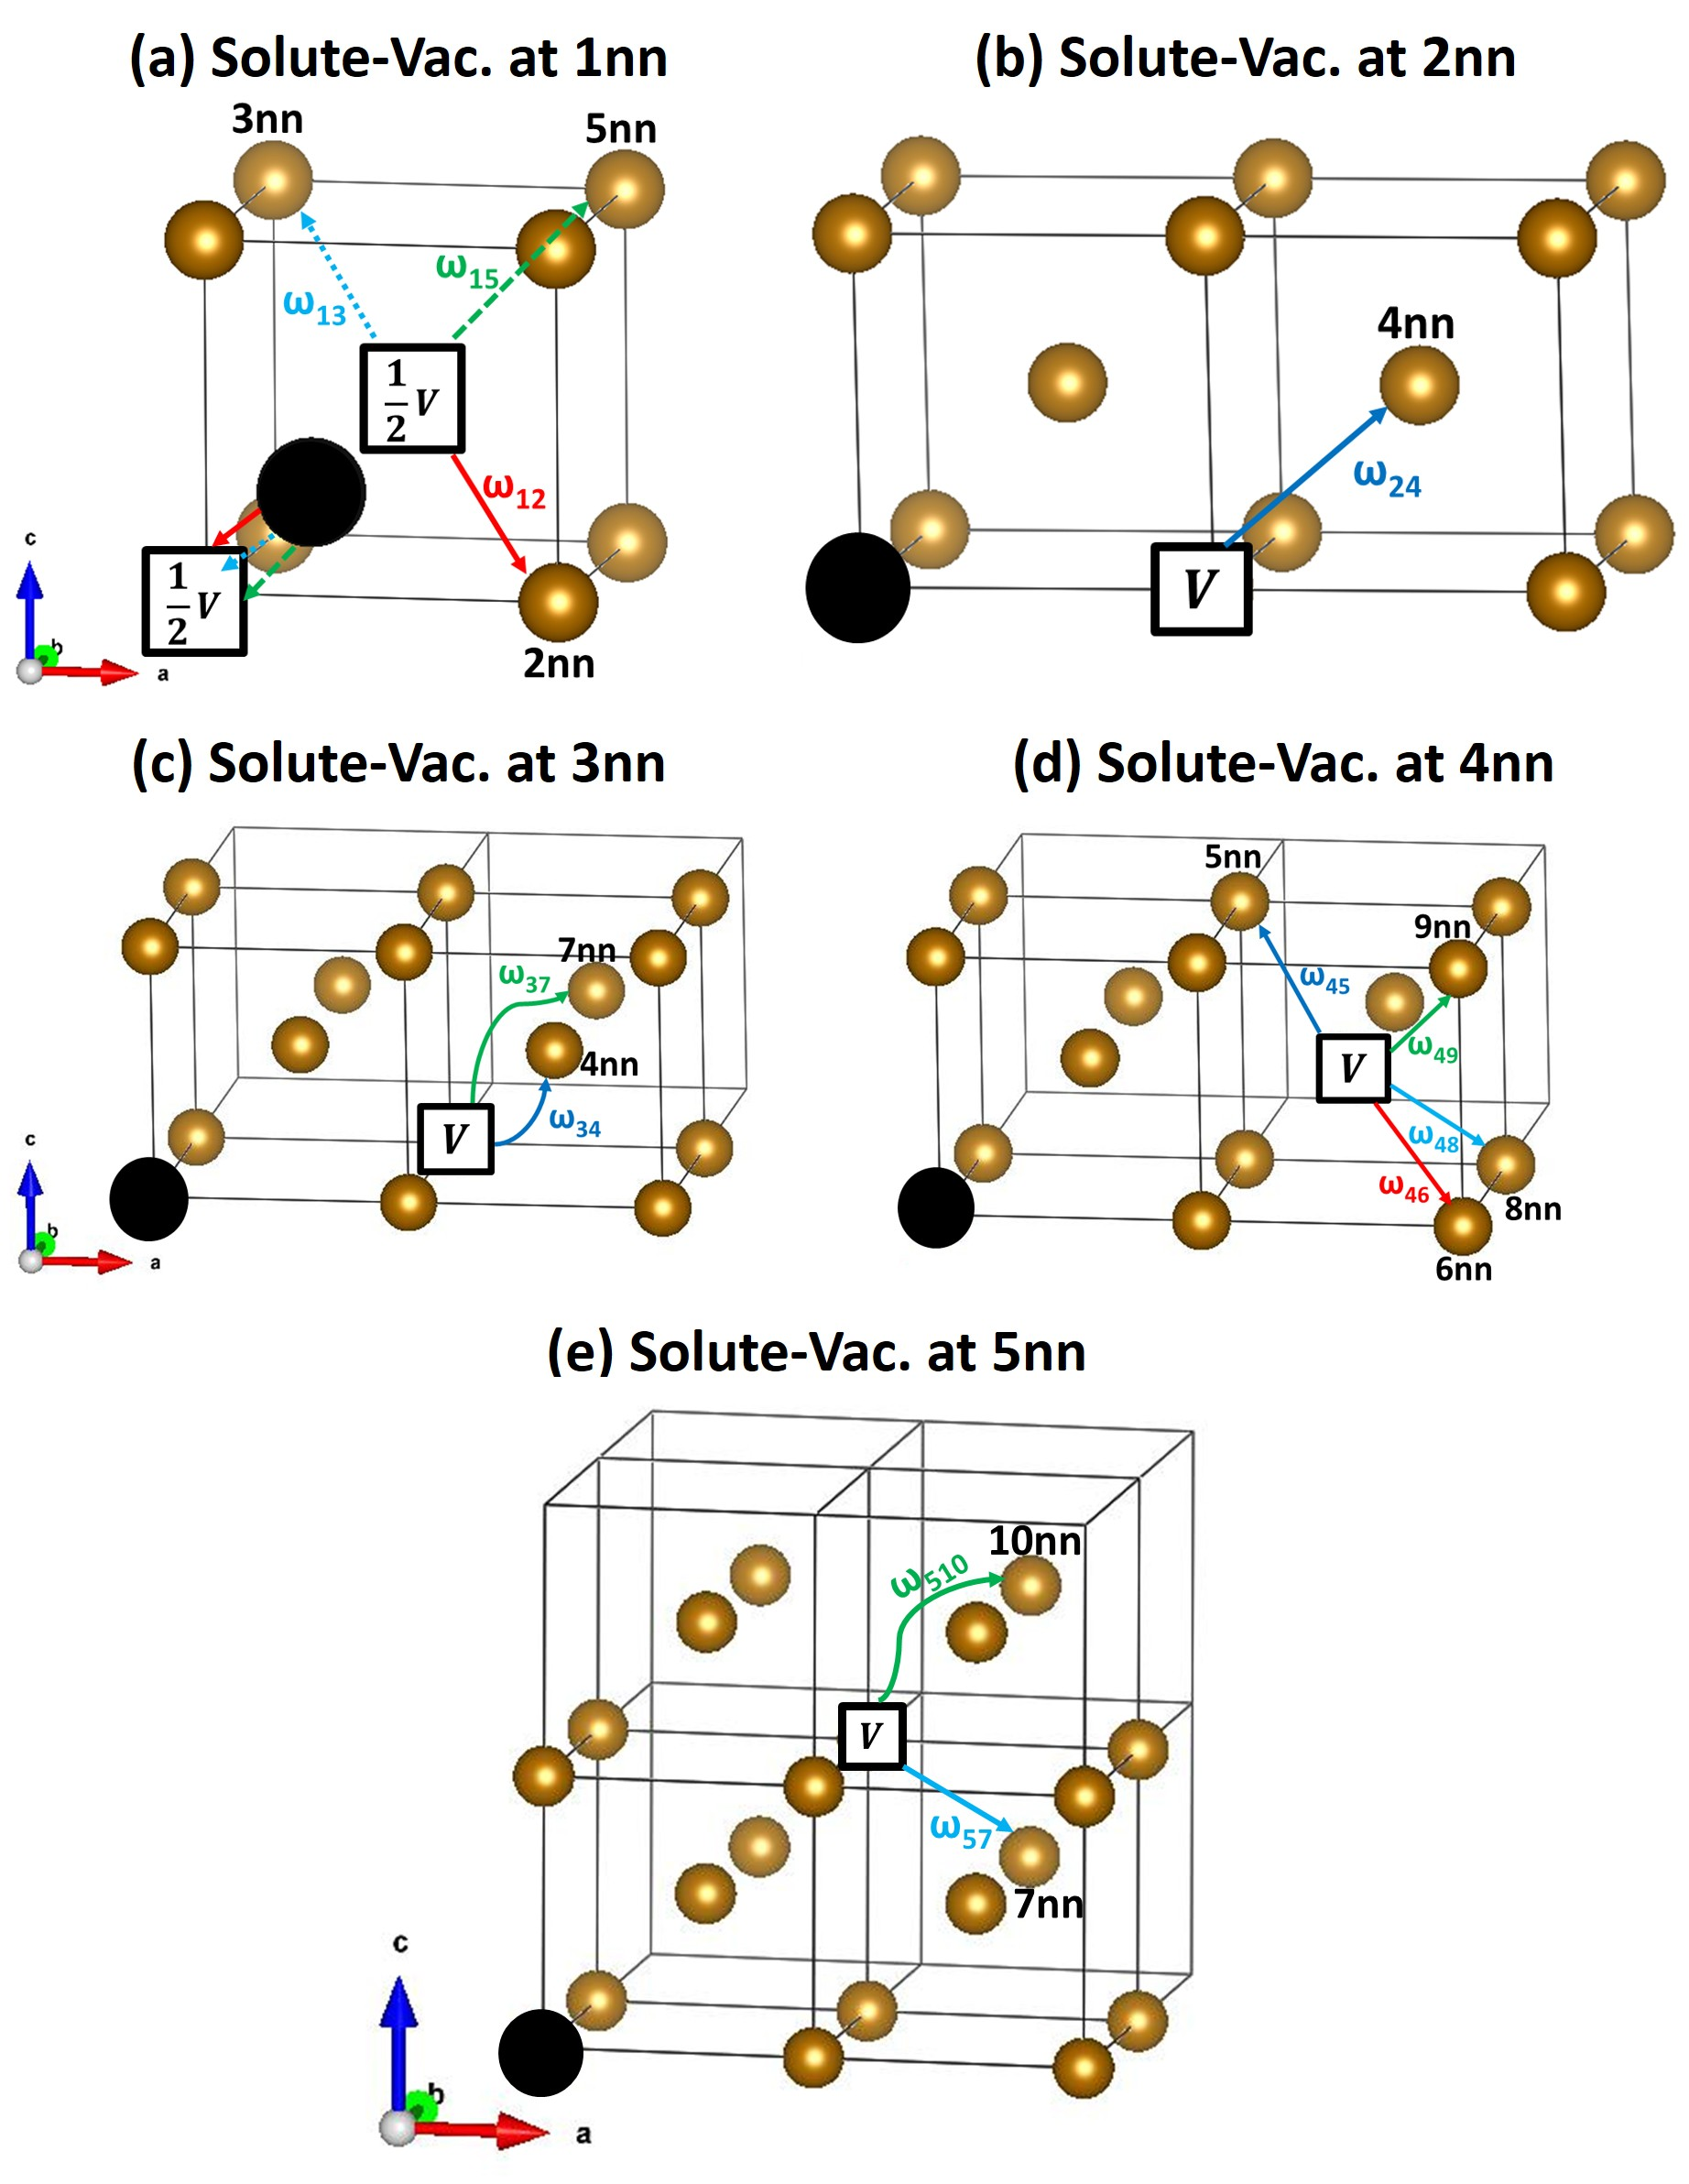
\includegraphics[width=0.7\linewidth]{jumps_all_modified_arrows.jpg}
    \caption{(a) The three possible jumps for the vacancy-solute pair at the first-nearest neighbor configuration (1nn). The oversized solute atom (black sphere) is intermediate between the two half vacancies. The jumps are labeled $\omega_{if}$, where $i$ and $f$ are the initial and final configurations. In the jumps $\omega_{12}$, $\omega_{13}$, and $\omega_{15}$, the solute atom returns to the lattice site in the corner and the vacancy migrates to the 2nn, 3nn, or 5nn site, respectively. (b) The jump, $\omega_{24}$, for the vacancy-solute pair at the second-nearest neighbor configuration (2nn). Similarly, the jumps starting from the 3nn, 4nn, and 5nn configurations are shown in (c), (d), and (e), respectively.}
    \label{fig:jumps}
\end{figure}


In this work, the formation, binding, and migration energies of vacancies and solute-vacancy pairs are calculated using DFT energetics. The vacancy formation energy, $E_{form}^{vac}$, is evaluated as follows:
\begin{equation}
\label{eq_Ef_vac}
   E_{form}^{vac} = E^{vac}_{defect}[(N-1)A] - \frac{N-1}{N} E_{perfect}[(N) A] 
\end{equation}
The terms $E_{perfect}[(N) A]$ and $E^{vac}_{defect}[(N-1)A]$ are the DFT energies of the perfect and defect-containing supercells, respectively. The number of atoms in the perfect supercell is $N$, and $A$ is the atomic species of the host atom. Similarly, the substitutional formation energy of a solute $B$, $E_{form}^{sub,B}$, and the formation energy of a solute-vacancy complex, $E_{form}^{sub-vac,B}$, are evaluated as follows:
\begin{equation}
\label{eq_Ef_sub}
    E_{form}^{sub,B} = E_{defect}^{sub}[(N-1)A + B] - \frac{N-1}{N}E_{perfect}[(N) A] - E_{B}
\end{equation}

\begin{equation}
\label{eq_Ef_vac_sub}
    E_{form}^{sub-vac,B} = E_{defect}^{sub-vac}[(N-2)A + B] - \frac{N-2}{N}E_{perfect}[(N) A] - E_{B}
\end{equation}
where $E_{defect}^{sub}[(N-1)A + B]$ and $E_{defect}^{sub-vac}[(N-2)A + B]$ are the DFT energies of supercells containing one substitutional atom and a substitutional-vacancy pair, respectively, of species $B$. The last term, $E_{B}$, is the DFT energy per atom for the species $B$ in its pure form at 0 K (i.e., face-centered cubic Ce and double hexagonal close-packed Nd). The solute-vacancy binding energy, $E_{bind}^{sub-vac,B}$, is given by:
\begin{equation}
\label{eq_Eb}
    E_{bind}^{sub-vac,B} = E_{form}^{vac} + E_{form}^{sub,B} - E_{form}^{sub-vac,B}
\end{equation}
In this expression, a positive binding energy denotes attraction and a negative binding energy is repulsion. 

In addition to the binding energies of various solute-vacancy pair configurations, it is also essential to determine the rates at which these configurations transition to others, i.e., their jump frequencies. According to transition state theory \cite{vineyard_frequency_1957}, the jump frequency, $\omega_{if}$, for a transition from an initial configuration $i$ to a final configuration $f$ at temperature $T$, depends on the migration energy, $E_{if}^{mig}$, and is given by:
\begin{equation}
\omega_{if} = \nu^{i\rightarrow f} \exp\left(-\frac{E_{if}^{mig}}{k_BT}\right)
\end{equation}

\noindent The migration energies, $E_{if}^{mig}$, are determined from the DFT-calculated energy differences between the ground state and the saddle point along the migration path. 

The attempt frequency for a transition from configuration $i$ to $f$, $\nu^{i\rightarrow f}$, is estimated using an approximate form of Vineyard's harmonic transition state theory \cite{vineyard_frequency_1957}:

\begin{equation} \nu^{i\rightarrow f} = \frac{\prod_{j}^{3N_{hop}} \nu^{i}_{j}}{\prod_{j}^{3N_{hop}-1} \nu^{s,i\rightarrow f}_j}. \end{equation}

\noindent Here, $N_{hop}$ is the number of hopping atoms, which equals 1 for single vacancy jumps. In this study, all attempt frequencies are assumed to be equal to the intrinsic attempt frequency of a vacancy in pure BCC Cr or BCC V. This assumption significantly reduces the computational expense and \DIFdelbegin \DIFdel{may only alter the transport coefficients }\DIFdelend \DIFaddbegin \DIFadd{is expected to introduce minor errors }\DIFaddend by a factor of 2-2.5 at most \DIFdelbegin \DIFdel{. 
}\DIFdelend \DIFaddbegin \DIFadd{in the transport coefficients as suggested by Wu et al. \cite{wu_high-throughput_2016}.
}\DIFaddend 

The vacancy concentration, $C_{V}$, is assumed to be that of the thermodynamic equilibrium and can be evaluated using the Boltzmann-like expression:
\begin{equation}
    C_{V} = \exp\left(-\frac{E_{form}^{vac}}{k_BT}\right) \exp\left(\frac{S_{form}^{vac}}{k_B}\right)
\end{equation}
where $k_B$ is the Boltzmann constant and $S_{form}^{vac}$ is the vacancy formation entropy. $S_{form}^{vac}$ \DIFdelbegin \DIFdel{is evaluated asfollows:
}\DIFdelend \DIFaddbegin \DIFadd{was computed using the harmonic approximation applied to atoms within the first and second nearest neighbor shells of the vacancy site to reduce the computational expense. Specifically, vibrational frequencies were obtained using VASP with \texttt{IBRION = 5}, allowing only $N = 14$ atoms to vibrate via selective dynamics, while the rest of the supercell was kept fixed. The entropy was evaluated as:
}\DIFaddend \begin{equation}
   S_{form}^{vac} = k_B \ln\left(\DIFdelbegin \DIFdel{\frac{\Pi^{3N-1}_j \nu_j^{perfect}}{\Pi^{3N-1}_j \nu_j^{def}}}\DIFdelend \DIFaddbegin \DIFadd{\frac{\prod^{3N}_j \nu_j^{perfect}}{\prod^{3N}_j \nu_j^{def}}}\DIFaddend \right).
\label{eq_entropy}
\end{equation}
where \DIFaddbegin \DIFadd{$\nu_j^{\text{perfect}}$ and $\nu_j^{\text{def}}$ denote }\DIFaddend the vibrational frequencies \DIFaddbegin \DIFadd{of the selectively dynamic atoms }\DIFaddend in the perfect and defective supercells\DIFdelbegin \DIFdel{are denoted by $\nu_j^{perfect}$, and $\nu_j^{def}$, respectively. }\DIFdelend \DIFaddbegin \DIFadd{, respectively. Since the surrounding atoms were fixed, rigid-body translational modes do not appear, and all $3N$ frequencies were included directly in the calculation.
}\DIFaddend 

\begin{comment}

\begin{table}[]
    \centering
    \begin{tabular}{|c|c|c|}
    \hline
       Notation & Distance ($a_0$) & Direction  \\
        \hline
       1nn &$\frac{\sqrt{3}}{2}$ & $<$1 1 1$>$ \\
       \hline
       2nn &1 & $<$1 0 0$>$ \\
       \hline
       3nn &$\sqrt{2}$ &$<$1 1 0$>$  \\
       \hline
       4nn &$\frac{\sqrt{11}}{2}$ & $<$3 1 1$>$ \\
       \hline
       5nn &$\sqrt{3}$ & $<$1 1 1$>$  \\
       \hline
       6nn &2 & $<$1 0 0$>$ \\
       \hline
       7nn &$\frac{\sqrt{19}}{2}$ & $<$3 3 1$>$ \\
       \hline
       8nn &$\sqrt{5}$ &$<$2 1 0$>$ \\
       \hline
       9nn &$\sqrt{6}$ & $<$2 1 1$>$  \\
       \hline
      10nn &$\frac{3\sqrt{3}}{2}$ & $<$1 1 1$>$  \\
      \hline
    \end{tabular}
    \caption{Vacancy-solute distances are represented in terms of the lattic constant ($a_0$)}
    \label{tab:my_label}
\end{table}
\end{comment}

\subsection{Evaluation of Transport Coefficients}

The DFT energetics obtained using the approach described in section \ref{sec:methods_energetics} are utilized to evaluate the Onsager transport coefficients, $L_{ij}$. The Onsager transport coefficients relate the flux $J_i$ of species $i$ to the chemical potential gradient $\mu_j$ of species $j$ according to the following relationship \citep{allnatt_atomic_2003}:

\begin{equation}
   J_i = -\sum_j{L_{ij} \frac{\nabla\mu_j}{k_B T}}. 
   \label{eq_onsager}
\end{equation}

The Onsager transport coefficients, $L_{ij}$, defined in Equation \ref{eq_onsager}, are evaluated assuming vacancy-mediated diffusion. Accordingly, there are two diffusing species: vacancies (V) and solutes (B). Accordingly, the $L_{ij}$ coefficients can then be expressed in matrix form and Equation \ref{eq_onsager} can be rewritten as:

\begin{equation}
\label{matrix_form_onsager}
    \begin{bmatrix}
        J_V \\
        J_B 
    \end{bmatrix}=\frac{-1}{k_B T}
    \begin{bmatrix}
    L_{VV} & L_{VB} \\
    L_{VB} & L_{BB}
    \end{bmatrix}
        \begin{bmatrix}
        \nabla\mu_V \\
        \nabla\mu_B
    \end{bmatrix}.
\end{equation}

\noindent The $L_{ij}$ coefficients are calculated using SCMF theory \citep{nastar_self-consistent_2000, nastar_mean_2005}, as implemented in the KineCluE code \citep{schuler_kineclue_2020}. Inputs to KineCluE include the binding energies of solute-vacancy pairs, the saddle point energies for possible transitions between the solute-vacancy pairs, and the attempt frequencies obtained from DFT calculations. KineCluE employs a cluster expansion approach \citep{schuler_kineclue_2020}, wherein transport coefficients are first calculated separately for clusters containing only vacancies, $L_{ij}^{(V)}$, and for clusters containing a vacancy-solute pair, $L_{ij}^{(VB)}$. The weighted contributions from these clusters are then combined as follows:

\begin{equation}
\label{eq_cluster_exp}
\begin{bmatrix}
L_{VV} & L_{VB} \\
L_{VB} & L_{BB}
\end{bmatrix}
=
C \Biggl(
f_V 
\begin{bmatrix}
{L_{VV}}^{(V)} & 0 \\
0 & 0 
\end{bmatrix}
+ f_{VB}
\begin{bmatrix}
{L_{VV}}^{(VB)} & {L_{VB}}^{(VB)} \\
{L_{VB}}^{(VB)} & {L_{BB}}^{(VB)}
\end{bmatrix}
\Biggr),
\end{equation}
where $C$ is the total concentration of sites occupied by vacancies or vacancy-solute pairs, and $f_V$, and $f_{VB}$ are the fractions of single vacancy and the vacancy-solute clusters, respectively. The quantities $C$, $f_V$, and $f_{VB}$ are calculated using the partition functions as explained in our previous works \cite{shousha2024first, shousha_vacancy-mediated_2024} and the partition functions are evaluated using KineCluE \citep{schuler_kineclue_2020}.

The obtained transport coefficients will be used to evaluate the solute diffusion coefficients, $D_B$ as follows:

\begin{equation}
\label{eq_solute_diffusivity}
    D_B = \frac{L_{BB}}{C_B}
\end{equation}
where $C_B$ is the concentration of the solute (B). It should be noted that $D_B$ is independent of solute concentration within the dilute limit assumption. The maximum solute concentration allowed in this dilute model is 0.185$\%$ and is dictated by the chosen kinetic range as explained in references \cite{messina_solute_2020,shousha_vacancy-mediated_2024,shousha2024first}.

The self-diffusion coefficient can be obtained similarly but the solute atom (B) is replaced with a tracer atom ($A^*$) that has the same energetics as a matrix atom ($A$) (i.e., migration barrier of $A^*$-vacancy exchange is equal to the vacancy migration energy and the binding energy of $A^*$-vacancy is zero for any configuration). Then, Equation \ref{eq_solute_diffusivity} becomes:
\begin{equation}
    D_{A^*} = \frac{L_{A^*A^*}}{C_{A^*}}
\end{equation}

The off-diagonal transport coefficients, $L_{VB}$, can also be used to analyze the flux coupling between vacancies and solute atoms. One key metric is the vacancy drag ratio ($G_V$), which indicates whether a solute diffuses in the same direction as the vacancy flux ($G_V > 0$, due to vacancy drag) or in the opposite direction ($G_V < 0$, known as the inverse Kirkendall effect, IKE \citep{marwick_segregation_1978}). The vacancy drag ratio is defined by Equation \ref{eq:drag}:

\begin{equation}
\label{eq:drag}
G_V = \frac{L_{VB}^{(VB)}}{L_{BB}^{(VB)}}
\end{equation}

Another important quantity, the partial diffusion coefficient ratio ($D_{pd}$), describes the relative diffusion speed and direction of a solute compared to the host atoms, taking into account flux coupling with vacancies \citep{messina_exact_2014,messina_solute_2020}. It is defined by Equation \ref{eq:pdc}:

\begin{equation}
\label{eq:pdc}
D_{pd} = \frac{(1-C_B)}{C_B} \frac{L_{VB}}{L_{AV}}
\end{equation}

The value of $D_{pd}$ provides insights into the behavior of solutes near vacancy sinks (e.g., grain boundaries) and their tendencies toward enrichment or depletion \citep{messina_exact_2014}. When $D_{pd} < 0$, $L_{VB} > 0$ and $L_{AV}$ is always negative. This indicates solute enrichment at vacancy sinks, driven by solutes diffusing in the same direction as the vacancy flux ($G_V > 0$), which is a signature of vacancy drag. For $D_{pd} > 1$, solute depletion occurs at sinks due to a favorable vacancy-solute exchange, with solutes moving in the opposite direction to the vacancy flux ($G_V < 0$) and diffusing faster than the host atoms. In the intermediate range $0 < D_{pd} < 1$, solute enrichment occurs at sinks even in the absence of vacancy drag ($G_V < 0$). In this case, both solute and host atoms move away from the sinks (opposite to the vacancy flux), but because solutes diffuse more slowly than the host atoms, they accumulate at the sinks \citep{messina_exact_2014}.

\FloatBarrier

\subsection{Density Functional Theory Computational Details}
\label{sec:methods:dft}
The projector-augmented wave method implemented in VASP \cite{kresse_ab_1993, kresse_efficient_1996} was used to perform DFT calculations. Spin-polarized calculations with collinear magnetic moments were used to generate antiferromagnetic BCC Cr. The relaxed BCC Cr structure has a total magnetic moment of zero and the local magnetic moments on Cr sites are $\pm$1.10 $\mu$B per atom.
In the case of V, we employed a non-spin polarized setting to model the BCC V structure.
The Perdew-Burke-Ernzerhof generalized gradient approximation \cite{perdew_generalized_1996} was utilized for exchange-correlation functions. Supercells with 128 atoms were generated through the $4\times4\times4$ duplication of the conventional BCC unit cell. A plane-wave cutoff energy of 450 eV was applied in all calculations. The Brillouin zone sampling was performed using a $4\times4\times4$ $\Gamma$-centered k-points mesh. The Methfessel-Paxton smearing method was employed with a width of 0.2 eV  \cite{methfessel_high-precision_1989}. 
The convergence criteria of total energies and forces during geometry relaxations were set to $10^{-6}$ eV, and 0.01 eV/\AA, respectively. All geometry relaxations for defect-containing supercells were conducted under a fixed volume constraint. The climbing image nudged elastic band (CI-NEB) method \cite{henkelman_climbing_2000} using three intermediate images was used to calculate the migration barriers of the jumps starting from the 1nn configuration, while one-image CI-NEB calculations were performed for all the other jumps.

Phonon calculations to determine attempt frequencies and vacancy formation entropies were carried out by computing the force constants using the finite-differences approach implemented in VASP \cite{kresse_ab_1993, kresse_efficient_1996}. Atomic displacements of 0.02 {\AA} were applied to evaluate the Hessian matrix \cite{hafner_ab-initio_2008}.

\section{Results}

\subsection{Lanthanide-Vacancy Interactions}

To ensure the accuracy of the DFT calculations, the bulk properties and defect energetics of pure BCC Cr and V were evaluated and are presented in Table \ref{tab:bulk_prop_cr_v}. The calculated lattice constants and defect properties are in reasonable agreement with values reported in the literature. Minor discrepancies were observed, such as a higher vacancy formation energy and attempt frequency in Cr, which can be attributed to the antiferromagnetic state assumed in this study. 
%Here, Cr is modeled as antiferromagnetic, whereas previous studies \cite{yang_significant_2023, SHANG2016128, nguyen_bcc_2006} employed non-spin-polarized calculations, neglecting the influence of magnetism on defect properties.


\begin{table}[]
    \centering
    \caption{The lattice constants and the defect properties in BCC Cr and V are presented in comparison to previous results in the literature \citep{yang_significant_2023,nguyen_bcc_2006,SHANG2016128,BOEV201714,fattahpour_understanding_2022, DENG201655}}
    \setlength{\tabcolsep}{7.5pt} % Default value: 6pt
    \renewcommand{\arraystretch}{1.25} % Default value:
    \resizebox{\textwidth}{!}{
    \begin{tabular}{|c|c|c|}
    \hline
         &BCC Cr & BCC V  \\
         \hline
         \begin{tabular}{c}
                \\
              %\hline
              $a_0$ (\AA) \\
              $E_{form}^{vac}$ (eV) \\
              $E_{mig}^{vac}$ (eV)  \\
              $S_{form}^{vac}$ (k$_B$) \\
              $\nu$ (THz) 
         \end{tabular} & \begin{tabular}{c|c} 
             This work & Literature  \\
             %\hline
             2.86 & 2.83\cite{yang_significant_2023}, 2.85\cite{nguyen_bcc_2006}  \\
             3.00 & 2.64\cite{nguyen_bcc_2006}, 2.73\cite{yang_significant_2023}, 2.79\cite{SHANG2016128} \\
             1.17 & 0.91\cite{nguyen_bcc_2006}, 0.89\cite{yang_significant_2023}, 0.90\cite{SHANG2016128}\\
             3.30 & 2.25\cite{fattahpour_understanding_2022} \\
             7.4  & 2.01\cite{fattahpour_understanding_2022}
         \end{tabular} & \begin{tabular}{c|c}
             This work & Literature  \\
             %\hline
             3.03 & 3.04\cite{nguyen_bcc_2006} \\
             2.36 & 2.51\cite{nguyen_bcc_2006}, 2.48\cite{SHANG2016128}, 2.44\cite{BOEV201714}\\
             0.50 & 0.62\cite{nguyen_bcc_2006}, 0.46\cite{SHANG2016128} \\
             2.46 & 2.76 \cite{DENG201655}  \\
             4.4 & 3.09 \cite{DENG201655}  \\
         \end{tabular} \\
         \hline
     \end{tabular}}
    \label{tab:bulk_prop_cr_v}
\end{table}

\FloatBarrier

\begin{comment}
    \begin{table}[]
    \centering
    \caption{The lattice constants and the defect properties in BCC Cr and V are presented in comparison to previous results in the literature: $^a$:\citep{nguyen_bcc_2006}, $^b$:\citep{yang_significant_2023}, $^c$:\citep{SHANG2016128}, $^d$:\citep{BOEV201714},$^e$:\citep{fattahpour_understanding_2022} }
    \begin{tabular}{|c|c|c|}
    \hline
         &BCC Cr & BCC V  \\
         \hline
         \begin{tabular}{c}
                \\
              %\hline
              $a_0$ (\AA) \\
              $E_{form}^{vac}$ (eV) \\
              $E_{mig}^{vac}$ (eV)  \\
              $S_{form}^{vac}$ (k$_B$) \\
              $\nu$ (THz) 
         \end{tabular} & \begin{tabular}{c|c} 
             This work & Literature  \\
             %\hline
             2.86 & 2.85$^a$  \\
             3.00 & 2.64$^a$, 2.73$^b$, 2.79$^c$ \\
             1.17 & 0.91$^a$, 0.89$^b$, 0.90$^c$ \\
             3.30 & 2.25$^e$ \\
             7.4  & 2.01$^e$
         \end{tabular} & \begin{tabular}{c|c}
             This work & Literature  \\
             %\hline
             3.03 & 3.04$^a$ \\
             2.36 & 2.51$^a$, 2.48$^c$, 2.44$^d$ \\
             0.50 & 0.62$^a$, 0.46$^c$ \\
             2.46 &  \\
             4.4 &  \\
         \end{tabular} \\
         \hline
     \end{tabular}
    \label{tab:bulk_prop_cr_v}
\end{table}
\end{comment}


Table \ref{tab:configurations_binding_cr_v} lists the calculated solute-vacancy binding energies. Notably, the Nd-vacancy binding energy for the 5nn configuration in both Cr and V systems is omitted, as the 5nn configuration is found to be unstable and spontaneously relaxes to the first-nearest-neighbor (1nn) configuration. In contrast, the 5nn configuration remains stable for Ce-vacancy pairs. As a result, jumps such as $\omega_{15}$, $\omega_{45}$, $\omega_{57}$, and $\omega_{510}$ in the Cr-Nd and V-Nd systems are excluded from the transport coefficient calculations.

The solute-vacancy binding energies are also visualized in Figure \ref{fig:binding_energies_cr_v}, highlighting a strong attractive binding at the 1nn configuration for both Cr and V systems. Beyond the 1nn, the binding energy decreases significantly at the 2nn configuration and approaches zero for the 3nn and beyond. Furthermore, lanthanide-vacancy binding energies are generally stronger in Cr than in V, particularly at the 1nn and 2nn configurations. Additionally, Nd exhibits stronger binding with vacancies than Ce in both systems. This suggests that Nd substitutionals introduce a higher lattice stress and are less stable than Ce in the BCC Cr and V lattices. To verify this, the stress tensor of relaxed supercells with substitutional atoms under a constant volume constraint was analyzed. The residual stress induced by Ce and Nd substitutionals was found to be 10.16 kbar and 17.94 kbar, respectively, in BCC Cr, and 7.02 kbar and 13.13 kbar, respectively, in BCC V. These observations are further supported by the calculated substitutional formation energies, $E_{form}^{sub, B}$. For Ce and Nd in BCC Cr, $E_{form}^{sub, B}$ values are 3.13 and 5.04 eV, respectively, while for Ce and Nd in BCC V, they are 1.09 and 2.65 eV, respectively. The higher formation energies and residual stresses associated with Nd likely explain why the 5nn configuration is stable for Ce but not for Nd. \DIFdelbegin \DIFdel{The }\DIFdelend \DIFaddbegin \DIFadd{It should also be noted that while the stress tensor data could also be used to perform elastic corrections to solute-defect binding energies, as outlined by Varvenne et al. \cite{varvenne_point_2013, varvenne_elastic_2017}, such corrections were not applied in this work. Instead, our use of the stress tensor is limited to qualitative comparisons of lattice distortion. The elastic correction scheme is a useful post-processing method to mitigate finite-size effects and may be explored in future work.
The }\DIFaddend complete set of migration barriers for the jumps depicted in Figure \ref{fig:jumps} is provided in Table \ref{tab:migration_barriers_cr_v} in \ref{appendix:migration_barriers}.




\begin{figure}
    \centering
    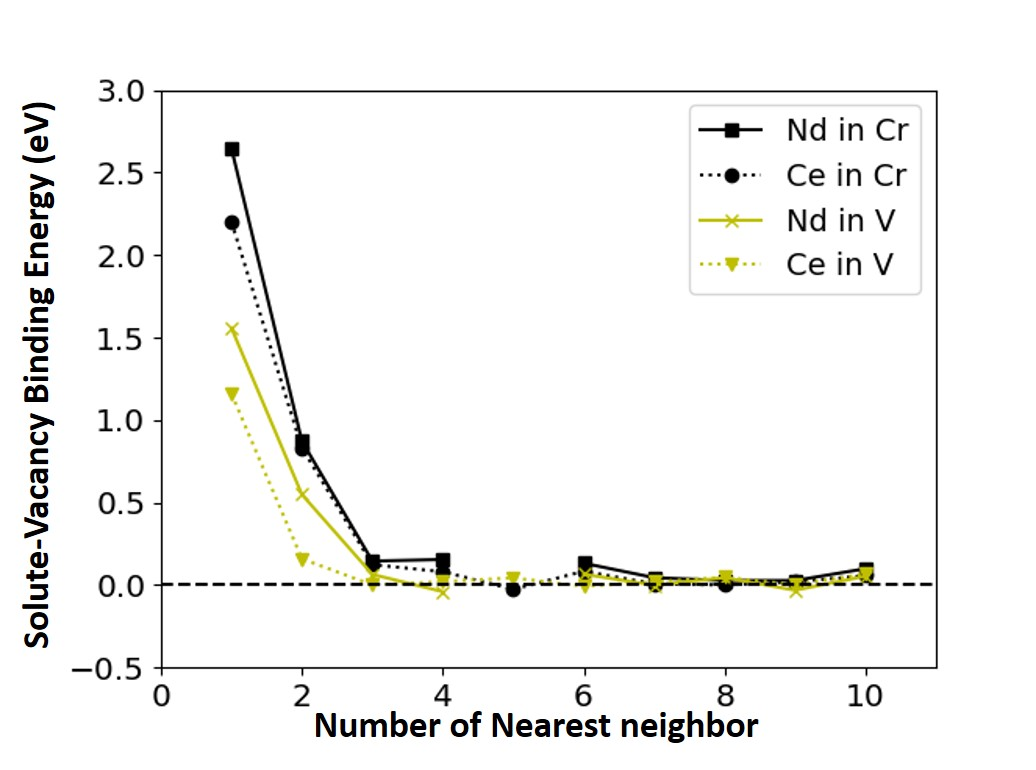
\includegraphics[width=0.9\linewidth]{BE_cr_v.jpg}
    \caption{Solute-vacancy binding energies in BCC Cr and V with separation distances ranging from first nearest neighbor (1nn) to the tenth nearest neighbor (10nn). Positive binding energies indicate attraction and negative binding energies are repulsion.}
    \label{fig:binding_energies_cr_v}
\end{figure}

\begin{table}[h!]
    \centering
    \caption{Notations, separation distances, orientations, binding energies of vacancy-solute pairs considered in this work. Vacancy-solute distances (d) are represented in terms of the lattice constant ($a_0$). The distances shown are between lattice sites in the unrelaxed crystal structure and not the distance after the ionic relaxation. All binding energies are in units of eV. Values with the superscript ($^a$) are from ref. \citep{yang_significant_2023}.}
    \begin{tabular}{|c|c|c|c|c|c|c|}
    \hline
       Notation & d ($a_0$) & Direction&  $E_{bind}^{Ce-vac} (Cr)$ & $E_{bind}^{Nd-vac} (Cr)$ &$E_{bind}^{Ce-vac}$ (V)&$E_{bind}^{Nd-vac}$ (V) \\
        \hline
       1nn &$\frac{\sqrt{3}}{2}$ & $<$1 1 1$>$ & 2.201 &2.646 &1.159 &1.557 \\
       &&&2.61$^a$ &$2.42^a$ & & \\
       \hline
       2nn &1 & $<$1 0 0$>$ &0.832 &0.872 &0.159 &0.549 \\
       &&&0.89$^a$ &0.75$^a$ && \\
       \hline
       3nn &$\sqrt{2}$ &$<$1 1 0$>$  &0.123 &0.145 &0.001 &0.065 \\
       &&&0.14$^a$ & 0.12$^a$&& \\
       \hline
       4nn &$\frac{\sqrt{11}}{2}$ & $<$3 1 1$>$ & 0.080 &0.155 &0.021 &-0.041 \\
       &&&0.13$^a$ & 0.12$^a$ && \\
       \hline
       5nn &$\sqrt{3}$ & $<$1 1 1$>$  &-0.027 & - &0.043 & -\\
       &&&-0.06$^a$ &-0.07$^a$ && \\
       \hline
       6nn &2 & $<$1 0 0$>$ &0.084 &0.132 &-0.007 &0.066 \\
       \hline
       7nn &$\frac{\sqrt{19}}{2}$ & $<$3 3 1$>$ &0.007 &0.045 &0.019 &-0.002 \\
       \hline
       8nn &$\sqrt{5}$ &$<$2 1 0$>$ &0.000 &0.027 &0.047 &0.044 \\
       \hline
       9nn &$\sqrt{6}$ & $<$2 1 1$>$  &0.019 &0.027 &0.001 &-0.032 \\
       \hline
      10nn &$\frac{3\sqrt{3}}{2}$ & $<$1 1 1$>$ &0.057 &0.099 &0.067 &0.053 \\
      \hline
    \end{tabular}
    \label{tab:configurations_binding_cr_v}
\end{table}


\begin{comment}
    
\begin{table}[]
    \centering
    \caption{Migration barriers of $\omega_{ij}$ jumps in eV. The values in parentheses are previous DFT results from ref. \cite{yang_significant_2023} for Ce and Nd in BCC Cr using non-spin polarized calculations.}
    \begin{tabular}{|c|c|c|c|c|}
    \hline
      Jump &Cr-Ce &Cr-Nd &V-Ce  &V-Nd  \\
      \hline
       $\omega_{12}$  &2.581 (3.04) &2.961 (2.97)&1.449 &1.737 \\
       $\omega_{21}$  &1.213 (1.32) &1.187 (1.30) &0.448 &0.728 \\
       \hline
       $\omega_{13}$  &2.810 (2.76) &2.991 (2.64)&1.312 &1.509 \\
       $\omega_{31}$  &0.732 (0.29) &0.4891 (0.34)&0.153 &0.016 \\
       \hline
       $\omega_{15}$  &2.624 (2.71)&-  (2.54)&1.131 &- \\ 
       $\omega_{51}$  &0.397 (0.04)&-  (0.06)&0.015 &- \\
       \hline
       $\omega_{24}$  &1.377 (1.22)&1.350 (1.13)&0.445 &0.801 \\ 
       $\omega_{42}$  &0.626 (0.27)&0.632 (0.50)&0.307 &0.212 \\
       \hline
       $\omega_{34}$  &1.199 &1.235 &0.440 &0.536 \\ 
       $\omega_{43}$  &1.156 &1.244 &0.460 &0.431 \\
       \hline
       $\omega_{37}$ &1.153 &1.156 &0.543 &0.530 \\ 
       $\omega_{73}$  &1.037 &1.056 &0.563 &0.464 \\
       \hline
       $\omega_{45}$ &1.126 &- &0.506 &- \\ 
       $\omega_{54}$ &1.019 &- &0.529 &- \\
       \hline
       $\omega_{46}$ &1.087 &1.140 &0.515 &0.441 \\ 
       $\omega_{64}$ &1.091 &1.117 &0.487 &0.547 \\
       \hline
       $\omega_{48}$ &1.126 &1.182 &0.452 &0.450 \\ 
       $\omega_{84}$  &1.046 &1.054 &0.478 &0.534 \\
       \hline
       $\omega_{49}$ &1.149 &1.198 &0.437 &0.470 \\ 
       $\omega_{94}$  &1.088 &1.071 &0.417 &0.479 \\
       \hline
       $\omega_{57}$ &1.126 &- &0.483 &- \\ 
       $\omega_{75}$  &1.159 &- &0.459 &- \\
       \hline
       $\omega_{510}$ &1.141 &- &0.482 &- \\ 
       $\omega_{105}$  &1.225 &- &0.506 &- \\
       \hline
    \end{tabular}
    \label{tab:migration_barriers_cr_v}
\end{table}
\end{comment}

\FloatBarrier
\subsection{Lanthanide Diffusion Coefficients}
The calculated solute diffusivities are plotted versus the inverse temperature in Figure \ref{fig:diff_cr_v} and fitted to an Arrhenius expression ($D = D_0 \exp(-Q/k_BT)$). The diffusivities of Ce and Nd in HCP Zr from our previous work \cite{shousha2024first} are also plotted for comparison. \DIFaddbegin \DIFadd{To focus on the temperature range relevant to interdiffusion barrier applications, only values between 625 K and 1000 K are shown in Figure \ref{fig:diff_cr_v}.
}\DIFaddend First, the diffusion of Ce and Nd in BCC Cr is examined. As shown in Figure \ref{fig:diff_cr_v}, the diffusivities of Nd and Ce in BCC Cr are significantly lower than those in HCP Zr. The high activation energies can explain this for vacancy-mediated diffusion in BCC Cr, which are 3.39 eV for Ce and 3.32 eV for Nd. These values are related to the relatively high vacancy formation energy in Cr (3.00 eV) compared to that of HCP Zr (2.00 eV). Additionally, the vacancy migration energy in pure BCC Cr is 1.17 eV, which is higher than that in HCP Zr (0.57 eV for basal jumps and 0.65 eV for pyramidal jumps). Therefore, the observed lower diffusivities in BCC Cr \DIFdelbegin \DIFdel{are expected }\DIFdelend \DIFaddbegin \DIFadd{compared to those in HCP Zr are consistent with expectations }\DIFaddend for any substitutional solute diffusing via \DIFdelbegin \DIFdel{a }\DIFdelend \DIFaddbegin \DIFadd{the }\DIFaddend vacancy mechanism, not just lanthanides\DIFdelbegin \DIFdel{like Ce and Nd}\DIFdelend \DIFaddbegin \DIFadd{. This conclusion remains valid even when using vacancy formation and migration energies from non-magnetic DFT studies \cite{nguyen_bcc_2006, yang_significant_2023, SHANG2016128} as listed in \Cref{tab:bulk_prop_cr_v}}\DIFaddend .

\begin{figure}[h!]
    \centering
    \DIFdelbeginFL %DIFDELCMD < 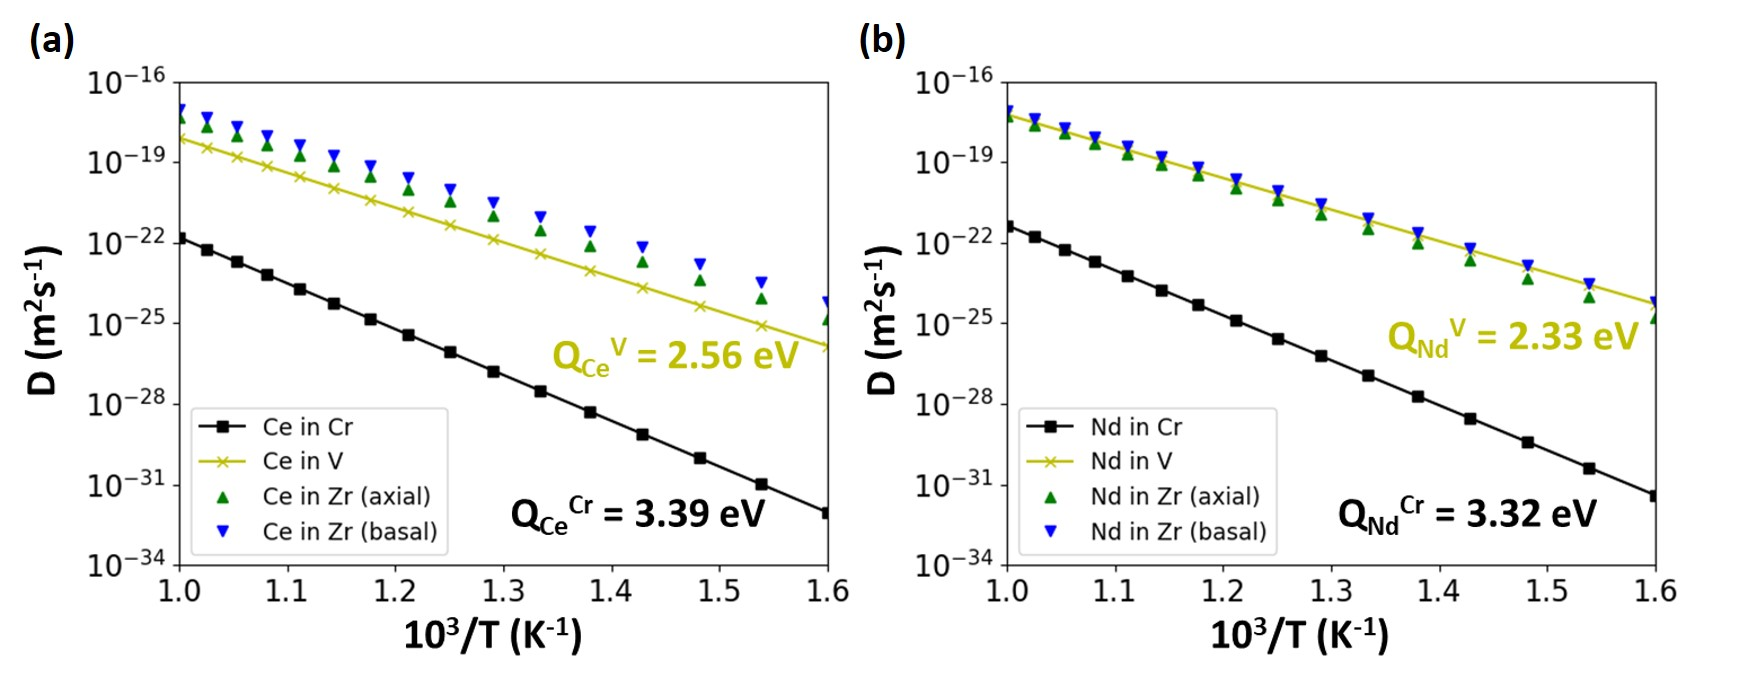
\includegraphics[width=0.9\linewidth]{diffusivities_cr_v.jpg}
%DIFDELCMD <     %%%
\DIFdelendFL \DIFaddbeginFL 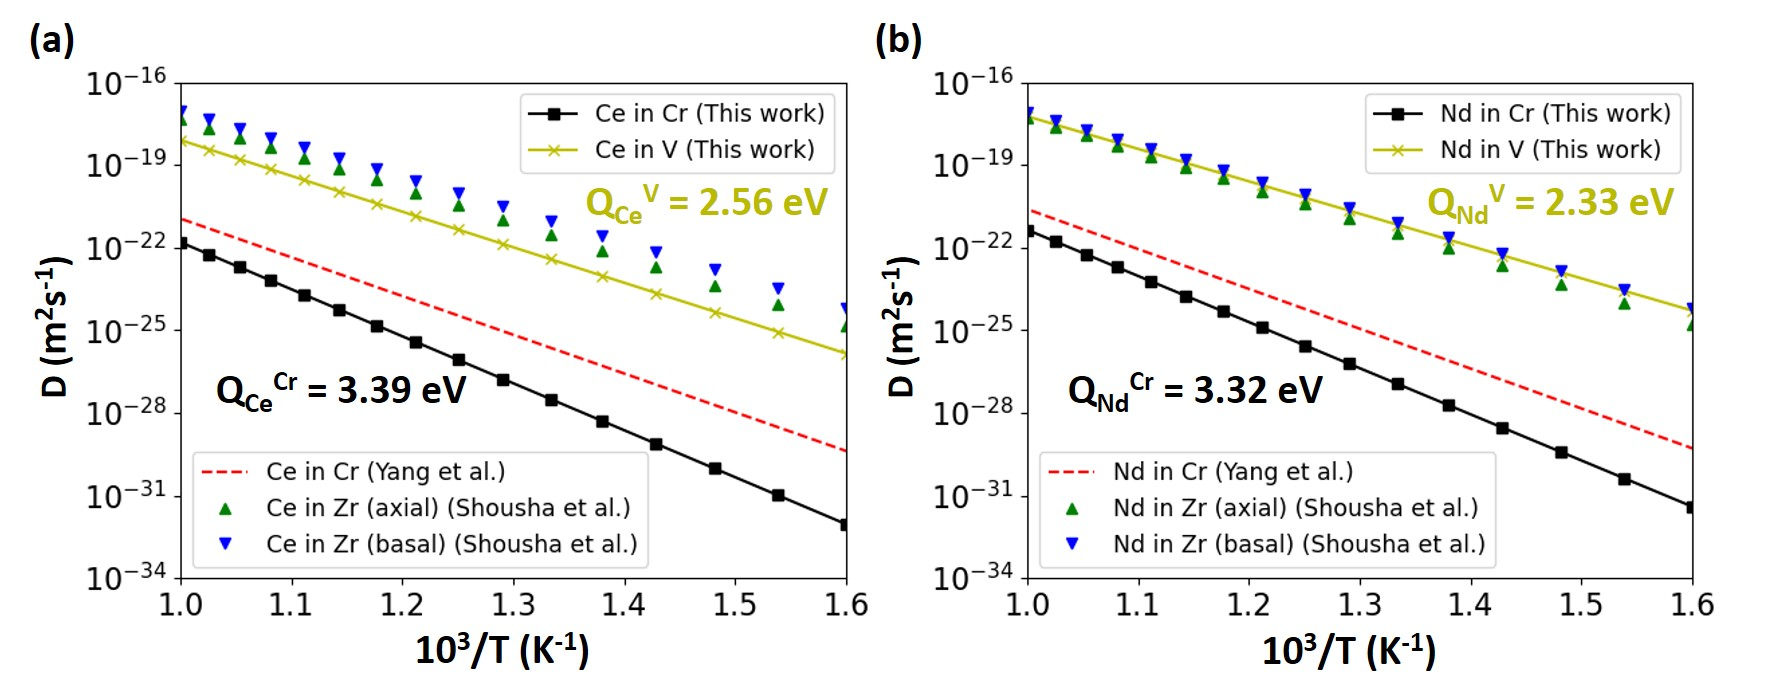
\includegraphics[width=0.9\linewidth]{diffusivities_cr_v_yang.jpg}
    \DIFaddendFL \caption{The diffusion coefficients of (a) Ce, and (b) Nd in BCC Cr and BCC V are plotted versus inverse temperature. The diffusion coefficients in \DIFaddbeginFL \DIFaddFL{BCC Cr and }\DIFaddendFL HCP Zr from ref. \DIFaddbeginFL \DIFaddFL{\citep{yang_significant_2023} and }\DIFaddendFL \cite{shousha2024first}\DIFaddbeginFL \DIFaddFL{,respectively, }\DIFaddendFL are also plotted for comparison.}
    \label{fig:diff_cr_v}
\end{figure}

In the case of Ce and Nd diffusion in BCC V, the diffusivities are comparable to those in HCP Zr. However, unlike HCP Zr, where Ce and Nd exhibit nearly identical diffusion coefficients, Ce diffuses more slowly than Nd in BCC V. The activation energies for Ce and Nd in BCC V are 2.56 and 2.33 eV, respectively. 

The fitted activation energies ($Q$) and prefactors ($D_0$) for self- and solute diffusion are presented in Table \ref{tab:activation_energies_Cr_V}, along with comparisons to results from the available literature. The activation energies for self-diffusion in Cr obtained in this work are relatively higher than those reported in previous DFT studies \citep{yang_significant_2023,nguyen_bcc_2006, fattahpour_understanding_2022}. Similarly, the activation energies for the diffusion of Ce and Nd in BCC Cr are also higher than those reported by Yang et al. \cite{yang_significant_2023}\DIFdelbegin \DIFdel{.
}\DIFdelend \DIFaddbegin \DIFadd{, resulting in lower diffusivities in our results compared to Yang et al. as shown in \Cref{fig:diff_cr_v}. However, our calculated value for self-diffusion activation energy (4.17 eV) in BCC Cr shows improved agreement with experimental values (4.51 and 4.20 eV) \cite{mundy1976isotope, mundy1981self} in contrast to earlier DFT studies did not account for the antiferromagnetic ground state of Cr at 0 K.
(See \Cref{tab:activation_energies_Cr_V}), supporting the validity of our approach.
}\DIFaddend 

\begin{table}[h!]
    \centering
    \caption{The fitted activation energies, $Q$, and the prefactors, $D_0$, in BCC Cr and V are presented compared with the available results in the literature:  \cite{nguyen_bcc_2006}$^a$, \cite{yang_significant_2023}$^b$, \cite{fattahpour_understanding_2022}$^c$, \cite{mundy1976isotope}$^d$, \cite{mundy1981self}$^e$, \cite{ullmaier1991atomic}$^f$, \cite{segel1997vanadium}$^g$}
    \setlength{\tabcolsep}{7.5pt} % Default value: 6pt
    \renewcommand{\arraystretch}{1.25} % Default value:
    \resizebox{\textwidth}{!}{
    \begin{tabular}{|c|c|c|}
    \hline
        & BCC Cr & BCC V  \\
        \hline
       \begin{tabular}{c}
              \\
            Q (eV) (This work) \\
           Previous DFT \\
            Exp. \\
        \hline
         $D_0$ ($\times 10^{-6} m^2 s^{-1}$) (This work)\\
            Previous DFT \\
            Exp. \\
       \end{tabular} & \begin{tabular}{ccc}
           Cr (self) & Ce & Nd  \\
           \hline
          4.17 &3.39 &3.32 \\
          3.55$^a$, 3.62$^b$, 3.68$^c$ &2.79$^b$ &2.87$^b$ \\
          4.51$^d$, 4.20$^e$ &- &- \\
           \hline
           12.0&18.9 &24.5 \\
           -&0.13$^b$ &0.72$^b$ \\
           97,000$^d$, 4600$^e$&- &- \\
        \end{tabular}
         & \begin{tabular}{ccc}
            V (self) & Ce & Nd  \\
            \hline
           2.86 &2.56 & 2.33 \\
           3.13$^a$ &- &- \\
           2.6$^f$, 3.20$^g$ &- &- \\
            \hline
            3.4&7.1 &3.8 \\
            -&- &- \\
           35.9$^g$&- &- \\
         \end{tabular}\\
         \hline
    \end{tabular}}
    \label{tab:activation_energies_Cr_V}
\end{table}

\DIFdelbegin \DIFdel{This discrepancy }\DIFdelend \DIFaddbegin \DIFadd{The discrepancy with Yang et al. \cite{yang_significant_2023} }\DIFaddend can be attributed to the higher vacancy formation and migration energies obtained in this work, which used the antiferromagnetic structure of BCC Cr. In contrast, studies in the literature used non-spin polarized calculations \citep{yang_significant_2023,nguyen_bcc_2006,SHANG2016128,fattahpour_understanding_2022}. For example, Yang et al. report vacancy formation and migration energies in BCC Cr that are 0.27 eV and 0.28 eV lower than the values calculated in this work, as shown in Table \ref{tab:bulk_prop_cr_v}. The sum of these differences, 0.55 eV, approximately matches the discrepancy in the activation energies for both self- and solute diffusion shown in Table \ref{tab:activation_energies_Cr_V}.

Since antiferromagnetic ordering is the ground state of BCC Cr at 0 K, performing spin-polarized DFT calculations with an antiferromagnetic configuration provides a more accurate representation. However, extrapolating point defect energetics, such as vacancy formation and migration energies, to temperatures above Cr's Néel temperature (312 K) \citep{bacon1969magnetic} is not rigorous, as finite-temperature effects, including the transition from antiferromagnetic ordering to paramagnetism, would need to be considered for a more accurate analysis. While corrections may be necessary at higher temperatures, addressing these effects falls beyond the scope of this study.

\DIFaddbegin \DIFadd{Finally, it is important to emphasize that our use of thermodynamic interactions extending up to the 5nn, in contrast to the 2nn limit used in the nine-frequency model by Yang et al. \cite{yang_significant_2023} does not account for the discrepancy observed in the BCC Cr results. To confirm this, our SCMF model was tested with a reduced thermodynamic interaction range limited to 2nn, excluding binding and migration energies beyond that range. The resulting activation energies differed by less than 1 meV in both BCC Cr and V, indicating that extending the interaction range does not significantly affect the diffusivity trends. However, including interaction up to the 5nn is necessary to accurately evaluate the off-diagonal transport coefficients ($L_{VB}^{VB}$) in \Cref{eq_cluster_exp} and vacancy drag ratios in \Cref{eq:drag}, which are presented in the next section. In our previous study on HCP Zr \cite{shousha2024first} , it was shown that vacancy drag ratios are sensitive to the choice of the thermodynamic range and that achieving converged results requires accounting for long-range solute-vacancy interactions.
}

\DIFaddend \FloatBarrier
\subsection{Vacancy Drag and Solute Segregation Tendencies}
\label{section_drag_cr_v}

To gain insight into the flux coupling between vacancies and solutes, $G_V$ and $D_{pd}$ were evaluated and plotted in Figure \ref{fig:drag_cr_v} and compared to the results in HCP Zr from ref. \cite{shousha2024first}.
\DIFaddbegin \DIFadd{The temperature range was extended up to 2000 K—approaching the melting points of Cr and V—in order to examine whether the solute segregation behavior undergoes a transition from vacancy drag at low temperatures to the inverse Kirkendall mechanism at high temperatures, as observed for lanthanides in HCP Zr \cite{shousha2024first}.
}\DIFaddend For Ce and Nd in Cr, a strong vacancy drag ($G_V >> 0$) occurs at all temperatures below the melting point. This behavior can be attributed to the strong attractive solute-vacancy binding at the 1nn and 2nn configurations in Cr, as shown in Figure \ref{fig:binding_energies_cr_v}. Consequently, $D_{pd}$ for Ce and Nd in BCC Cr remains negative, indicating a tendency for solute enrichment at vacancy sinks.

A similar trend is seen for Nd in BCC V, where vacancy drag and solute enrichment persist across all temperatures. However, in contrast to Ce and Nd in BCC Cr, the value of $G_V$ decreases and $D_{pd}$ increases with temperature. This difference is due to the significantly weaker Nd-vacancy binding in V compared to Cr, as illustrated in Figure \ref{fig:binding_energies_cr_v}. In the case of Ce in BCC V, where solute-vacancy binding is the weakest, the temperature dependence is more pronounced. A transition from the vacancy drag regime to the inverse Kirkendall regime occurs at 1300 K in BCC V, and the solute depletion regime occurs at temperatures above T = 1350 K.



\begin{figure}[h]
    \centering
    \DIFdelbeginFL %DIFDELCMD < 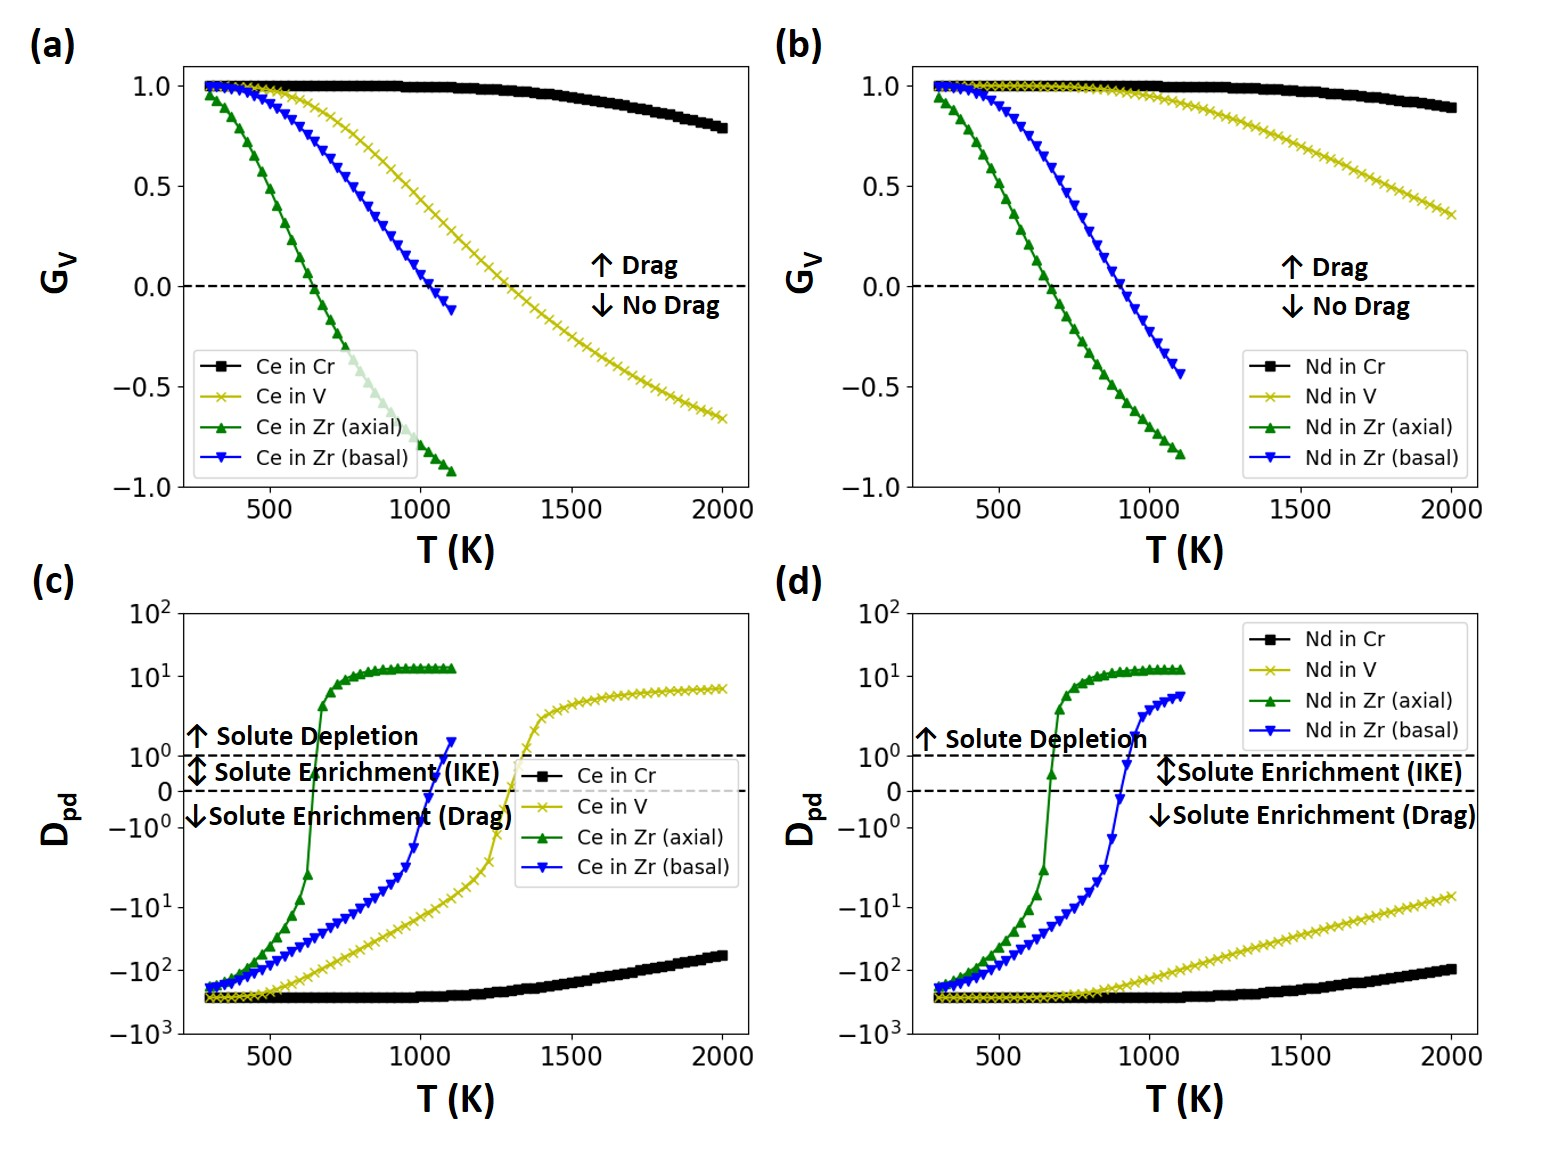
\includegraphics[width=0.99\linewidth]{drag_ratios_pdc_cr_v.jpg}
%DIFDELCMD <     %%%
\DIFdelendFL \DIFaddbeginFL 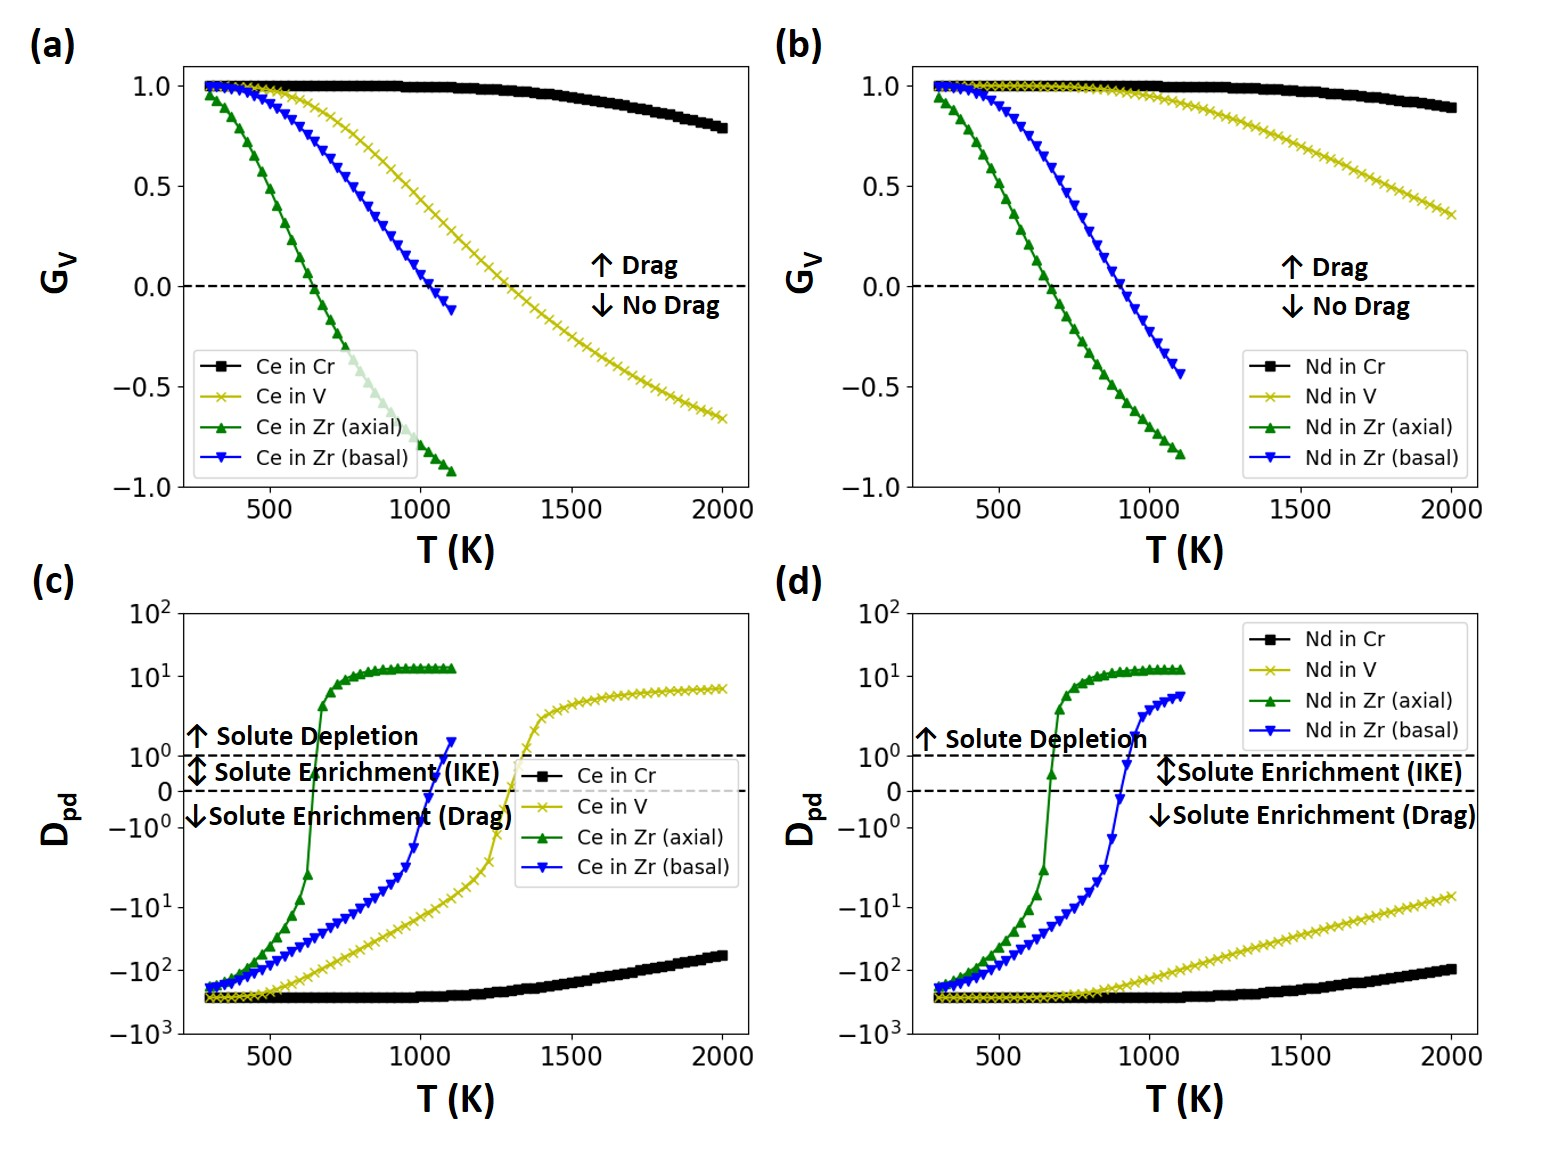
\includegraphics[width=0.9\linewidth]{drag_ratios_pdc_cr_v.jpg}
    \DIFaddendFL \caption{The vacancy drag ratios ($G_V$) of (a)Ce, and (b)Nd in BCC Cr and V compared to that in HCP Zr from ref. \cite{shousha2024first}. The partial diffusion coefficient ratios ($D_{pd}$) of Ce and Nd are plotted in (c) and (d), respectively.}
    \label{fig:drag_cr_v}
\end{figure}

\FloatBarrier
\section{Discussion}

\subsection{Vacancy-mediated diffusion vs. experimental measurements}

To evaluate the validity of the computed diffusivities, comparisons are made with available experimental data from the literature. As of the publication of this work, no direct diffusivity measurements of lanthanides in chromium or vanadium have been reported, except for a single V/Nd diffusion couple study by Helmreich \cite{helmreich_diffusion_2014}. However, the diffusivities reported in that study correspond to interdiffusion coefficients, which are derived from the concentration profiles of both V and Nd in the diffusion couple. In contrast, the diffusion coefficients computed in this work correspond to dilute lanthanide concentrations in BCC Cr and V and are analogous to tracer diffusion coefficients. Consequently, this section focuses on comparing the computed values with self- and impurity (though not necessarily lanthanide) tracer diffusion experiments available in the literature.

Experimental diffusivity measurements in pure chromium are scarce. Mundy et al. \cite{mundy1976isotope} measured the diffusivity of $^{51}$Cr and $^{48}$V radiotracers in single-crystal chromium. These diffusivities are plotted in Figure \ref{fig:diffusivities_vs_exp}(a) alongside the self-, Ce-, and Nd-diffusivities calculated in this work. Mundy et al. \cite{mundy1976isotope} suggested that the relatively high activation energies and diffusion prefactors in chromium may indicate that diffusion at these high temperatures is dominated by the divacancy mechanism. If this mechanism is indeed dominant, the discrepancy with our calculated self-diffusivity can be attributed to the fact that only the single-vacancy mechanism is considered in this work. The single vacancy mechanism is more relevant for the role of chromium as an interdiffusion barrier in sodium-cooled fast reactors, where a typical Cr liner or coating operates at temperatures in the range of 673-873 K \cite{beausoleil_fast_2022}. Experimental measurements of diffusivities in Cr at temperatures below 1000 K are not available in the literature.

\begin{figure}[htbp]
    \centering
    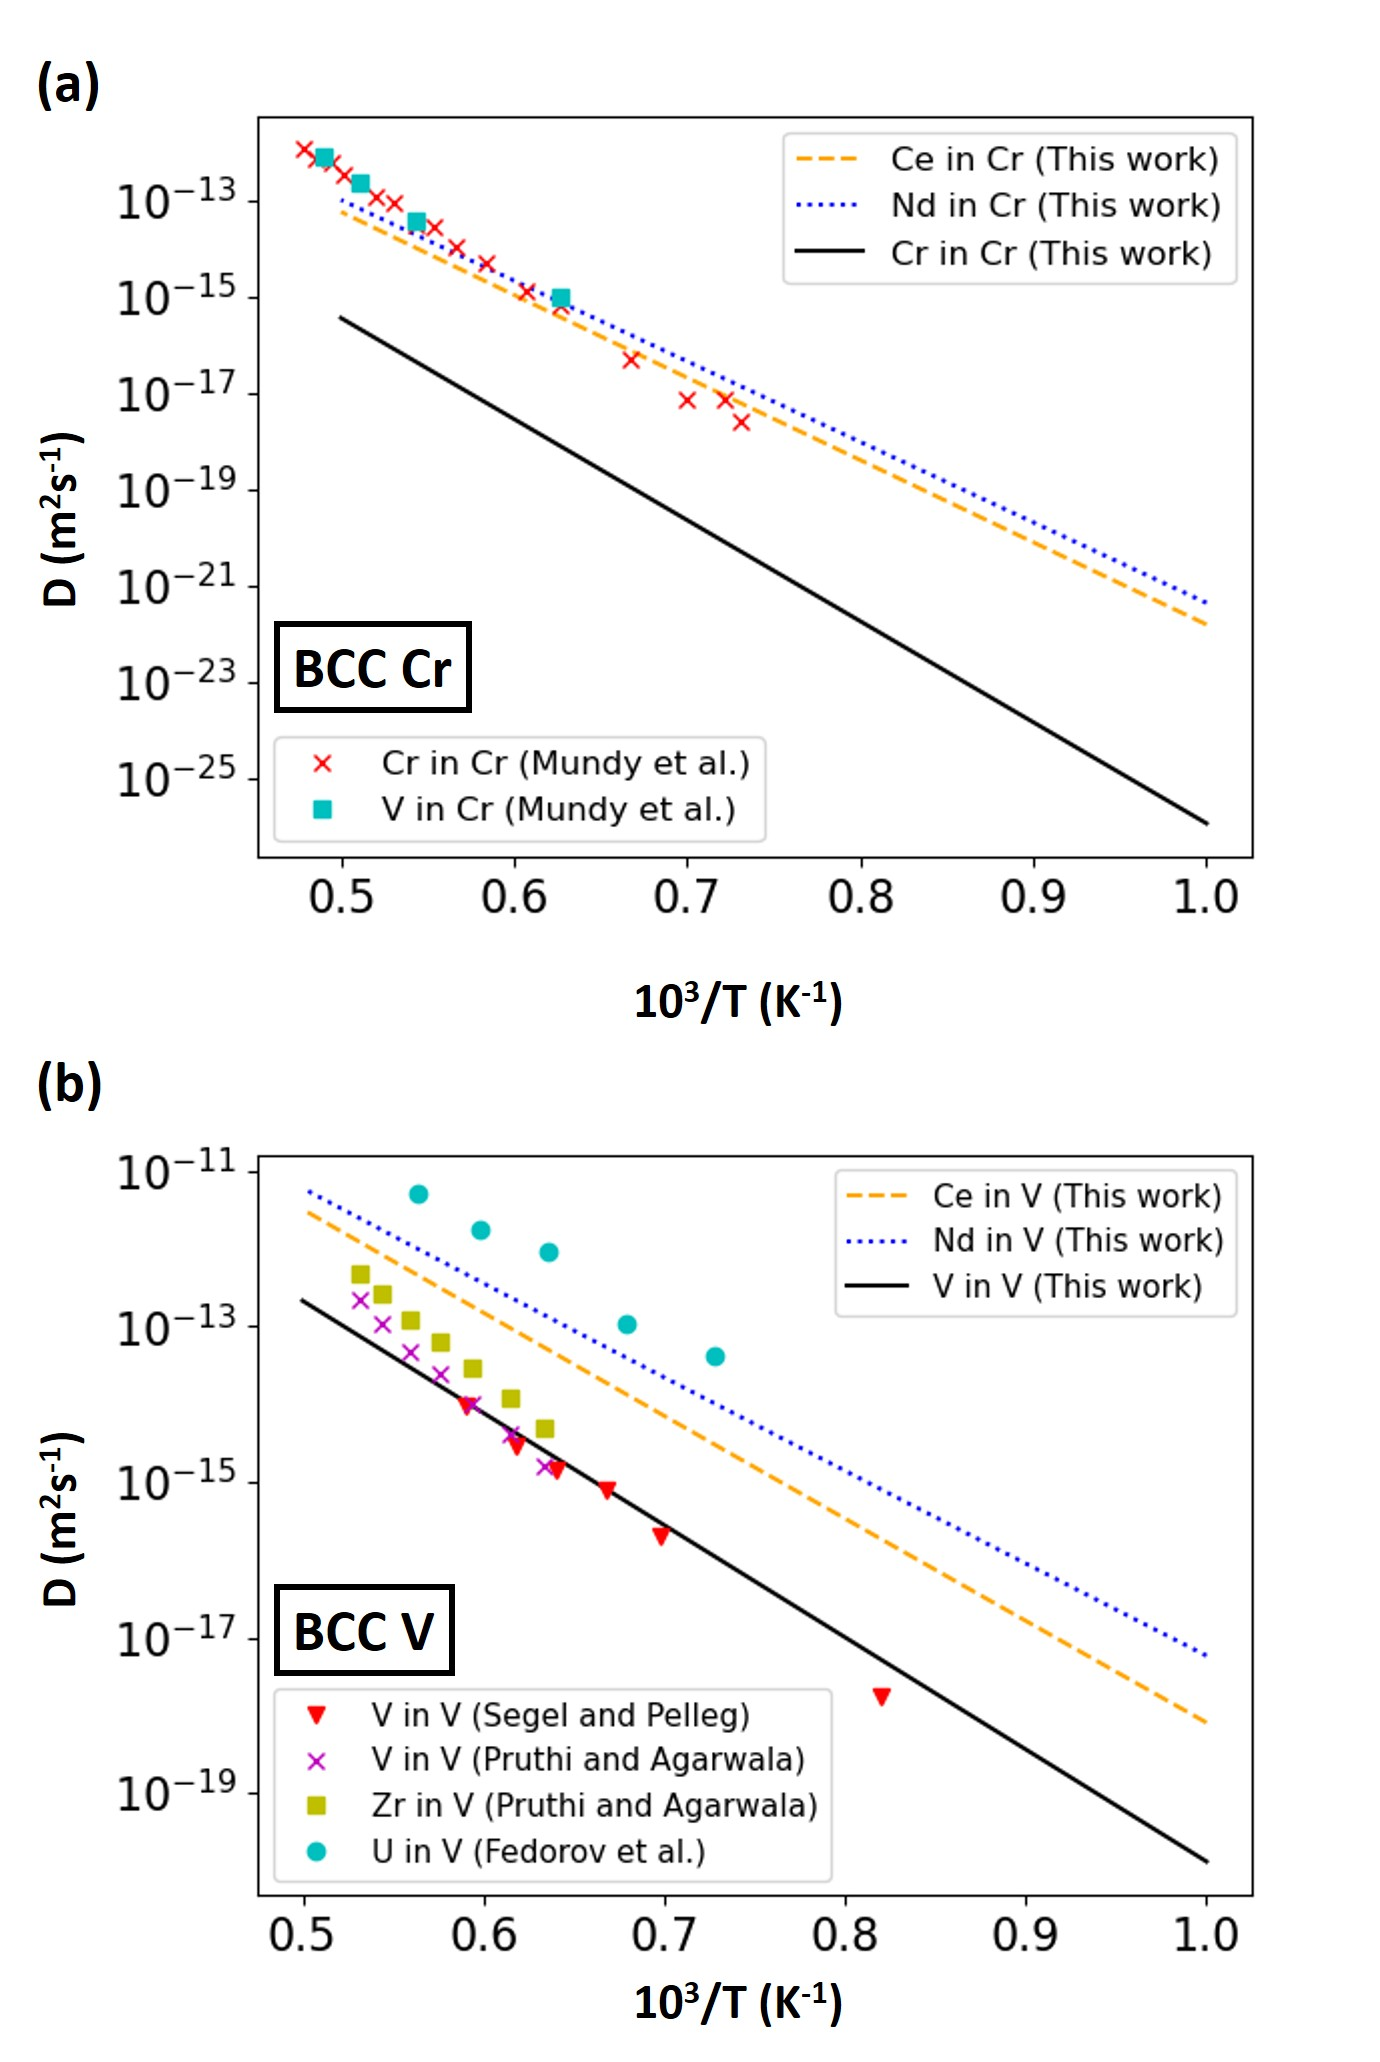
\includegraphics[width=0.825\linewidth]{experiments_cr_v.jpg}
    \caption{(a) The diffusivities of Ce, Nd, and self-diffusion in BCC Cr are plotted against inverse temperature and compared with experimental self- and impurity (V) diffusivities reported by Mundy et al. \cite{mundy1976isotope}. (b) The diffusivities of Ce, Nd, and self-diffusion in BCC V are plotted against inverse temperature and compared with experimental self- and impurity (Zr and U) diffusivities from \cite{segel1997vanadium, pruthi1984solute, fedorov1971diffusion}.}
    \label{fig:diffusivities_vs_exp}
\end{figure}

Similarly, the calculated self-, Ce-, and Nd-diffusivities in V are compared to experimental diffusion measurements \cite{segel1997vanadium, pruthi1984solute, fedorov1971diffusion} in Figure
\ref{fig:diffusivities_vs_exp}(b). The computed V self-diffusivities exhibit excellent agreement with measurements by Segel and Pelleg \cite{segel1997vanadium} using the $^{48}$V radiotracer, with a comparable activation energy of 3.20 eV to our fitted value of 2.86 eV. The agreement with self-diffusivity measurements by Pruthi and Agarwala \cite{pruthi1984solute} is also reasonable, as our diffusion coefficients are of the same order of magnitude as their reported values. However, their study reports a significantly higher activation energy of 4.03 eV \cite{pruthi1984solute}. The $^{95}$Zr diffusivity in vanadium, measured in the same study, is also shown in Figure
\ref{fig:diffusivities_vs_exp}(b). The experimental Zr diffusivity is slightly higher than the self-diffusivity, with an activation energy of 3.82 eV.

A particularly relevant comparison in Figure
\ref{fig:diffusivities_vs_exp}(b) is the $^{235}$U diffusion in V, as measured by Fedorov et al. \cite{fedorov1971diffusion}. Since actinides (such as U) and lanthanides (such as Ce and Nd) have larger atomic radii compared to transition metals such as V \cite{rahm2016atomic}, U can be considered an oversized solute similar to Ce and Nd. The U diffusivity in V, as measured by Fedorov et al. \cite{fedorov1971diffusion}, is significantly faster than self-diffusion, with an activation energy of 2.66 eV, which is comparable to our calculated values of 2.56 and 2.33 eV for Ce and Nd, respectively.

The significantly faster U diffusivity from experiments, along with our calculated lanthanide diffusivities in vanadium, compared to Zr and self-diffusivity, aligns with expectations for larger-sized solutes. This trend is consistent with the conclusions of Janotti et al. \cite{janotti2004solute}, who studied face-centered cubic metals and observed that larger solute atoms diffuse faster, contrary to the intuitive expectation that larger solutes would experience higher migration barriers. Theoretical calculations \cite{DENG201655,janotti2004solute} support this observation, showing that larger solutes tend to have lower migration barriers, which is consistent with the diffusion behavior of lanthanides and actinides in V discussed here.

%\FloatBarrier
\subsection{Chromium and Vanadium as interdiffusion barriers in nuclear fuels}
Comparing the diffusivities and segregation tendencies of lanthanides in BCC Cr, BCC V, and HCP Zr provides valuable insight into their suitability as candidate liners or coating materials. Under thermal equilibrium conditions, where the vacancy concentration is at its \DIFdelbegin \DIFdel{standard }\DIFdelend \DIFaddbegin \DIFadd{equilibrium }\DIFaddend level, lanthanide diffusivities in BCC Cr are significantly lower than in BCC V and HCP Zr. This suggests that Cr coatings may be particularly effective in mitigating FCCI by limiting lanthanide transport. However, under irradiation, vacancy concentrations increase, accelerating lanthanide substitutional diffusion in all liner materials. In such conditions, segregation behavior becomes a crucial factor. As proposed in our previous work \citep{shousha2024first}, an ideal diffusion barrier would exhibit solute depletion behavior ($D_{pd} > 1$), where lanthanides preferentially diffuse within the bulk rather than accumulating at vacancy sinks, such as the liner surface or grain boundaries, and, eventually, reaching the cladding.

Given the distinct segregation tendencies of lanthanides in BCC Cr and V compared to HCP Zr, it is expected that irradiation will promote greater lanthanide accumulation at vacancy sinks due to vacancy drag in BCC Cr and, to a lesser extent, in BCC V. In contrast, HCP Zr is likely to exhibit significantly lower lanthanide migration, as solute depletion, particularly in the axial direction, is more pronounced at typical liner operating temperatures (T $\approx$ 673–873 K) \citep{beausoleil_fast_2022}. Thus, while BCC metals—particularly Cr—offer lower lanthanide diffusivities under \DIFdelbegin \DIFdel{standard }\DIFdelend \DIFaddbegin \DIFadd{equilibrium }\DIFaddend conditions, their behavior under irradiation may favor the use of Zr liners. Further validation of this hypothesis is needed through rate theory and cluster dynamics models based on the transport coefficients calculated in this study and our previous work \citep{shousha2024first}, as well as through detailed characterization of microstructures and sink densities. Additionally, the role of self-interstitials under irradiation must be assessed. Other factors, including fabrication methods, mechanical performance, and interdiffusion reactions, should also be considered when selecting the optimal liner material to mitigate FCCI \cite{OH2024113102}.

\FloatBarrier
\section{Conclusion}
The diffusion coefficients of Ce and Nd in BCC Cr and V were determined using DFT energetics and SCMF analysis, assuming a vacancy-mediated diffusion mechanism. The results confirm that both lanthanides act as oversized solutes in the BCC Cr and V systems. The activation energies for Ce and Nd diffusion in BCC Cr were found to be 3.39 and 3.32 eV, respectively, indicating significantly slower diffusion compared to HCP Zr. In BCC V, the activation energies for Ce and Nd were 2.56 and 2.33 eV, respectively, which are comparable to the values reported for HCP Zr (2.36 and 2.34 eV for basal diffusion and 2.45 and 2.46 eV for axial diffusion) in our previous work \citep{shousha2024first}. These diffusion coefficients can serve as inputs for mesoscale and engineering-scale models to simulate FCCI in metallic fuels utilizing cladding coatings or liners. Furthermore, the vacancy drag ratios and partial diffusion coefficient ratios in BCC Cr and V indicate that vacancy drag and solute enrichment at sinks persist up to the melting point in BCC Cr. A similar trend is observed for Nd in BCC V, while for Ce in BCC V, this behavior remains significant up to approximately 1300 K—well above the typical operating temperatures of cladding liners in metallic fuels (673–873 K). This strong tendency for lanthanide enrichment at vacancy sinks in BCC Cr and V, particularly under irradiation, suggests that lanthanides may preferentially migrate from the BCC matrix to the liner surface or interfaces, increasing the risk of interaction with the cladding material. To better understand the irradiation-driven behavior of cladding liner materials, further investigation using rate theory and cluster dynamics models is necessary.

\FloatBarrier
\section{Acknowledgments}

This work was supported by grants from the U.S. Department of Energy, Office of Nuclear Energy (DOE-NE) (DE-NE0009271, Project 22-26632). This research made use of the resources of the High-Performance Computing Center at Idaho National Laboratory, which is supported by the Office of Nuclear Energy of the U.S. Department of Energy and the Nuclear Science User Facilities under Contract No. DE-AC07-05ID14517.

\appendix
\setcounter{table}{0}

\section{Vacancy-Solute Migration Barriers}
\label{appendix:migration_barriers}
The DFT-calculated migration barriers for solute-vacancy jumps visualized in Figure \ref{fig:jumps} are listed in Table \ref{tab:migration_barriers_cr_v}.

\begin{table}[]
    \centering
    \caption{Migration barriers of $\omega_{ij}$ jumps in eV. The values in parentheses are previous DFT results from ref. \cite{yang_significant_2023} for Ce and Nd in BCC Cr using non-spin polarized calculations.}
    \begin{tabular}{|c|c|c|c|c|}
    \hline
      Jump &Cr-Ce &Cr-Nd &V-Ce  &V-Nd  \\
      \hline
       $\omega_{12}$  &2.581 (3.04) &2.961 (2.97)&1.449 &1.737 \\
       $\omega_{21}$  &1.213 (1.32) &1.187 (1.30) &0.448 &0.728 \\
       \hline
       $\omega_{13}$  &2.810 (2.76) &2.991 (2.64)&1.312 &1.509 \\
       $\omega_{31}$  &0.732 (0.29) &0.4891 (0.34)&0.153 &0.016 \\
       \hline
       $\omega_{15}$  &2.624 (2.71)&-  (2.54)&1.131 &- \\ 
       $\omega_{51}$  &0.397 (0.04)&-  (0.06)&0.015 &- \\
       \hline
       $\omega_{24}$  &1.377 (1.22)&1.350 (1.13)&0.445 &0.801 \\ 
       $\omega_{42}$  &0.626 (0.27)&0.632 (0.50)&0.307 &0.212 \\
       \hline
       $\omega_{34}$  &1.199 &1.235 &0.440 &0.536 \\ 
       $\omega_{43}$  &1.156 &1.244 &0.460 &0.431 \\
       \hline
       $\omega_{37}$ &1.153 &1.156 &0.543 &0.530 \\ 
       $\omega_{73}$  &1.037 &1.056 &0.563 &0.464 \\
       \hline
       $\omega_{45}$ &1.126 &- &0.506 &- \\ 
       $\omega_{54}$ &1.019 &- &0.529 &- \\
       \hline
       $\omega_{46}$ &1.087 &1.140 &0.515 &0.441 \\ 
       $\omega_{64}$ &1.091 &1.117 &0.487 &0.547 \\
       \hline
       $\omega_{48}$ &1.126 &1.182 &0.452 &0.450 \\ 
       $\omega_{84}$  &1.046 &1.054 &0.478 &0.534 \\
       \hline
       $\omega_{49}$ &1.149 &1.198 &0.437 &0.470 \\ 
       $\omega_{94}$  &1.088 &1.071 &0.417 &0.479 \\
       \hline
       $\omega_{57}$ &1.126 &- &0.483 &- \\ 
       $\omega_{75}$  &1.159 &- &0.459 &- \\
       \hline
       $\omega_{510}$ &1.141 &- &0.482 &- \\ 
       $\omega_{105}$  &1.225 &- &0.506 &- \\
       \hline
    \end{tabular}
    \label{tab:migration_barriers_cr_v}
\end{table}

\FloatBarrier

\bibliographystyle{elsarticle-num} 
\bibliography{references}
\end{document}
